网络编程越来越受欢迎。大多数计算机都连接到互联网上,现在越来越多的应用程序依赖于此。从需要Internet连接的简单程序更新,到依赖稳定Internet连接的应用程序,网络编程正成为应用程序开发的必要部分。支持网络编程估计要推迟到以后的标准了,很可能要等到C++23。 \par
但我们可以通过处理网络应用程序提前做好准备。我们还将讨论网络的标准扩展,并看看在C++中支持网络会是什么样子。本章将集中讨论网络的主要原理和驱动设备间通信的协议。作为一个开发者,设计网络应用程序是一个强大的技能。 \par
开发人员经常面临的主要问题之一是应用程序的安全性。无论是与正在处理的输入数据相关,还是与使用经过验证的模式和实践进行编码相关,应用程序的安全性必须是第一位的。这对于网络应用程序尤为重要。本章中,我们还将深入探讨C++中进行安全编程的技术和最佳实践。 \par

本章中,我们将了解以下内容: \par

\begin{itemize}
	\item 计算机网络概论
	\item C++编写套接字和套接字编程
	\item 设计网络应用
	\item 理解C++中的安全问题
	\item 在项目开发中利用安全编程技术
\end{itemize}

\noindent\textbf{}\ \par
\textbf{编译器要求} \ \par
g++编译器需要添加编译选项 \texttt{-std=c++2a} 来编译本章的代码。可以从这里获取本章的源码文件:https:/​/github.​com/PacktPublishing/Expert-CPP \par

\noindent\textbf{}\ \par
\textbf{用C++进行网络编程} \ \par
两台计算机通过网络相互作用。计算机通过一种称为网络适配器或网络接口控制器的特殊硬件组件连接到Internet。安装在计算机上的操作系统提供与网络适配器一起工作的驱动程序,要支持网络通信,计算机必须有一个安装了支持网络堆栈的操作系统的网络适配器。所谓堆栈,我们指的是数据从一台计算机传输到另一台计算机时所经过的修改层。例如,在浏览器上打开一个网站会呈现通过网络收集到的数据。该数据以0和1的序列接收,然后转换为Web浏览器更容易理解的形式。分层在网络中是必不可少的,网络通信由符合我们将在这里讨论的OSI模型的几个层组成。网络接口控制器是支持OSI(Open System Interconnection)模型的物理链路层和数据链路层的硬件部件。 \par
OSI模型旨在对各种设备之间的通信功能进行标准化。设备在结构和组织上有所不同。这涉及到硬件和软件。例如,使用英特尔CPU、运行Android操作系统的智能手机与运行macOS Catalina的MacBook电脑是不同的。不同的不是上述产品背后的名称和公司,而是硬件和软件的结构和组织。为了消除网络通信中的差异,提出了一套标准化协议和内部通信功能作为OSI模型。我们前面提到的层次如下: \par

\begin{itemize}
	\item 应用层
	\item 表示层
	\item 会话层
	\item 传输层
	\item 网络层
	\item 数据链路层
	\item 物理层
\end{itemize}

可以简化成四个层: \par

\begin{itemize}
	\item 应用层:处理特定应用程序的细节。
	\item 传输层:提供两台主机之间的数据传输。
	\item 网络层:处理数据包在网络上的传输。
	\item 数据链路层:这包括操作系统中的设备驱动程序,以及计算机内部的网络适配器。
\end{itemize}

链路(或数据链路)层包括操作系统中的设备驱动程序,以及计算机中的网络适配器。 \par
为了理解这些层,我们假设正在使用一个用于消息传递的桌面应用程序,如Skype或Telegram。当你输入一条信息并点击发送按钮时,信息就会通过网络到达目的地。这个场景中,假设正在向计算机上安装了相同应用程序的朋友发送一条文本消息。从高级的角度来看,这似乎很简单,但这个过程是复杂的,即使是最简单的消息在到达目的地之前也要经历大量转换。首先,当您点击发送按钮时,文本消息将转换为二进制形式。网络适配器使用二进制文件进行操作。它的基本功能是通过媒体发送和接收二进制数据。除了通过网络发送的实际数据外,网络适配器还应该知道数据的目的地址。目标地址是附加到用户数据的许多属性之一。所谓用户数据,指的是输入并发送给朋友的文本。目的地址是你朋友计算机的唯一地址,输入的文本与目的地地址和其他发送到目标所必需的信息打包在一起,您朋友的计算机(包括网络适配器、操作系统和消息传递应用程序)接收并解包数据,包中包含的文本然后由消息传递应用程序呈现在屏幕上。 \par
本章开头提到的每一层OSI都将其特定的头添加到通过网络发送的数据中。下图描述了来自应用层的数据在移动到目的地之前,是如何与报头堆叠的: \par

\begin{center}
	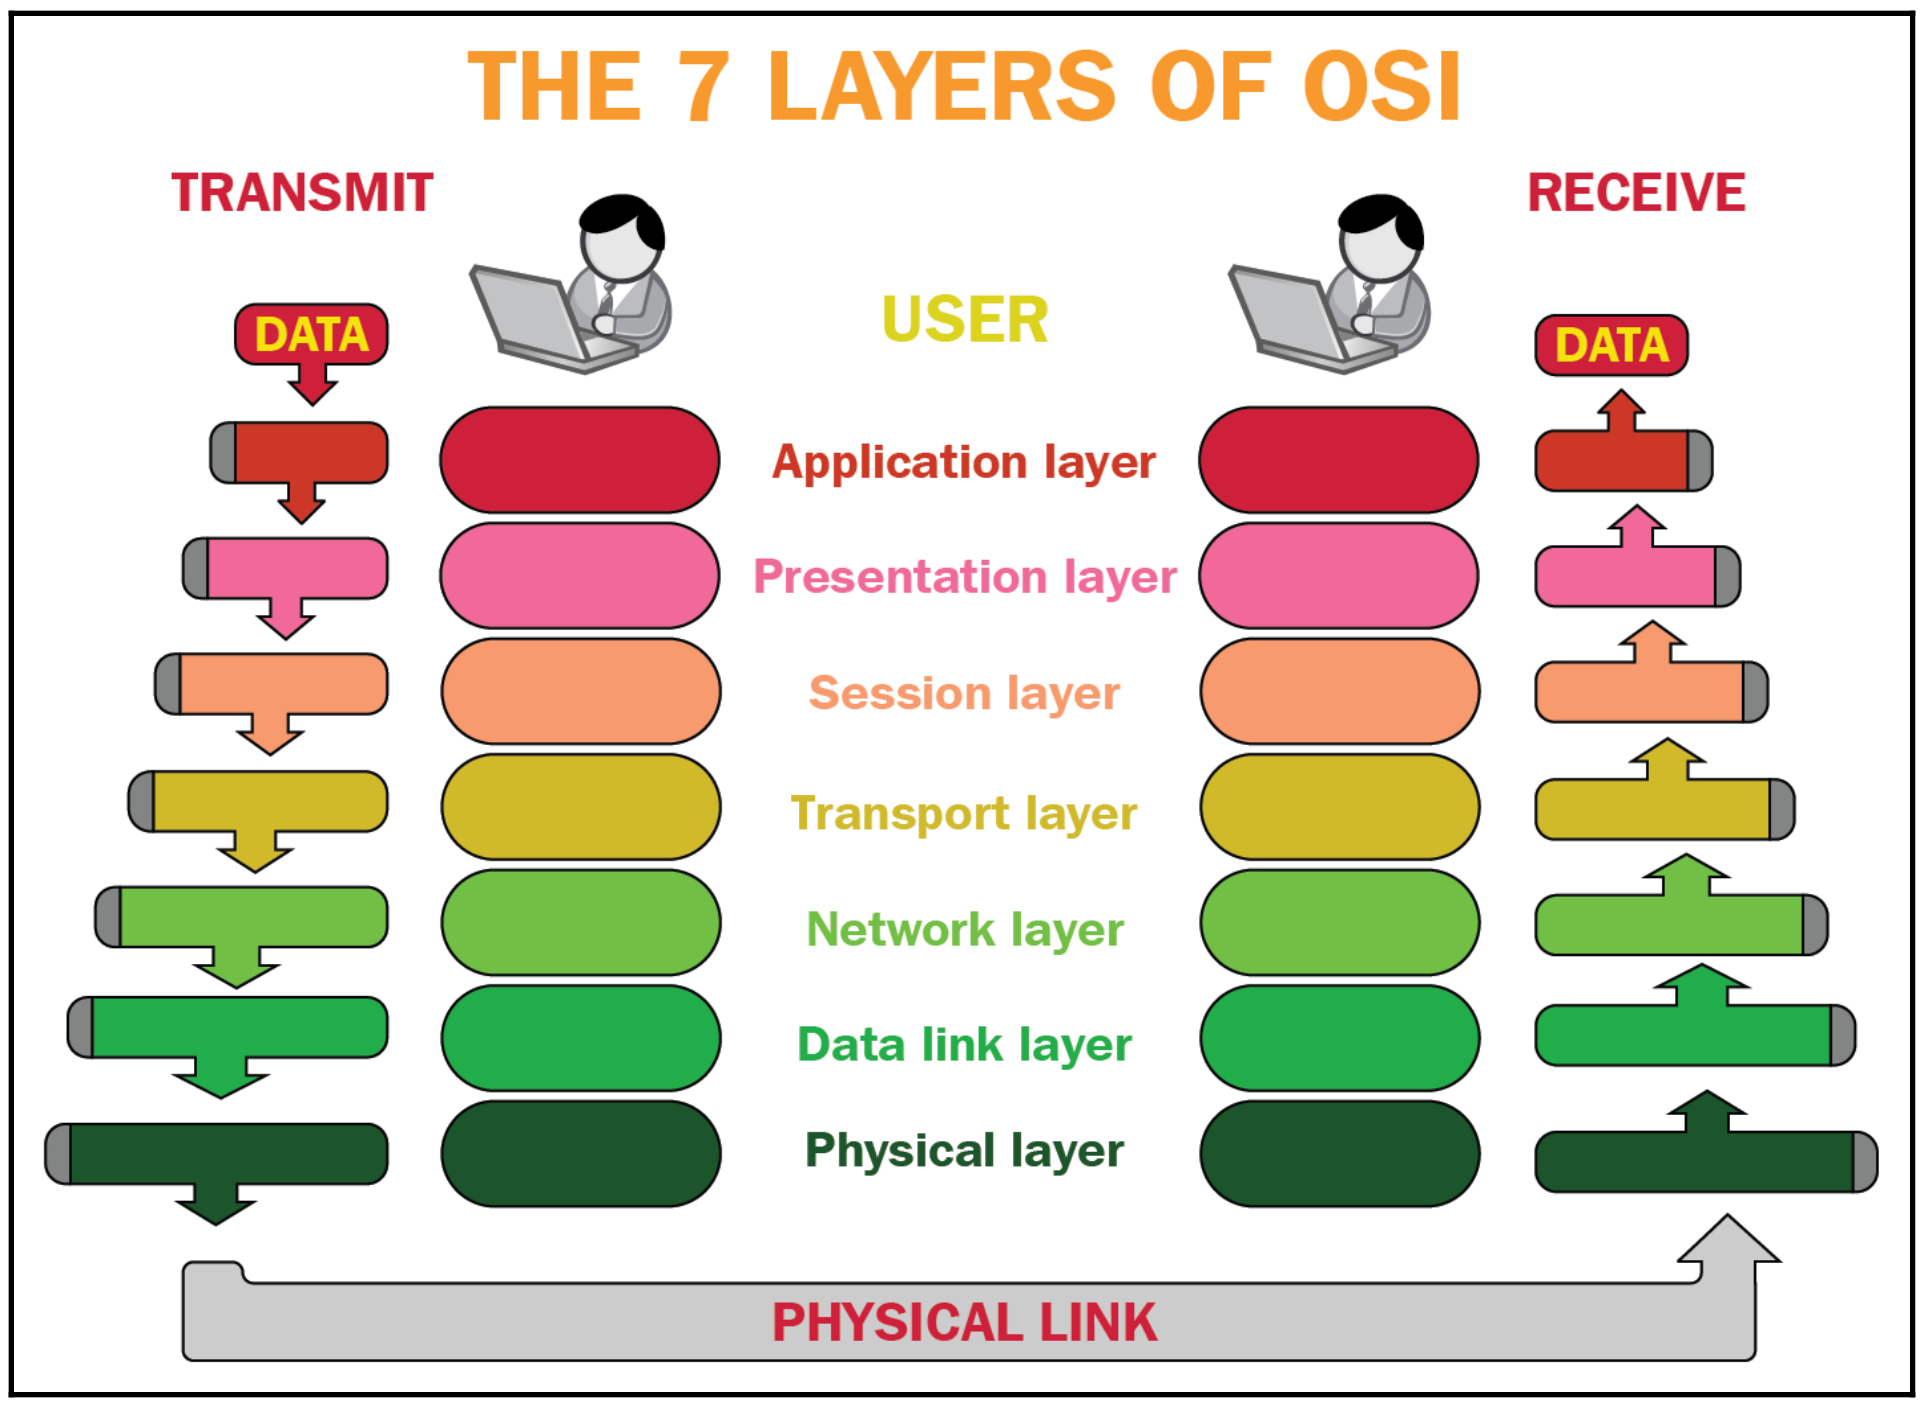
\includegraphics[width=1.0\textwidth]{content/Section-2/Chapter-12/1}
\end{center}

上图中的第一行(应用层)。数据是您在消息传递应用程序中输入的文本,以便将其发送给您的朋友。每一层数据都会向下传递,直到到物理层,数据打包与报头特定于OSI模型的每一层相对应。另一边的计算机接收和检索打包的数据。在每一层中,它删除特定于该层的头,并将包的其余部分移到下一层。最后,数据到达朋友的消息应用程序。 \par
作为开发者,我们主要关心的是编写能够通过网络发送和接收数据的应用程序,而不需要深入了解层的细节。然而,我们需要对层如何使用头文件在更高层次上增加数据的理解很少。让我们了解网络应用程序在实践中是如何工作的。 \par

\noindent\textbf{}\ \par
\textbf{底层的网络应用程序} \ \par
安装在设备上的网络应用程序通过网络与安装在其他设备上的其他应用程序进行通信。本章中,我们将讨论通过Internet协同工作的应用程序。下面的图表可以看到这种交流的上层概述: \par

\begin{center}
	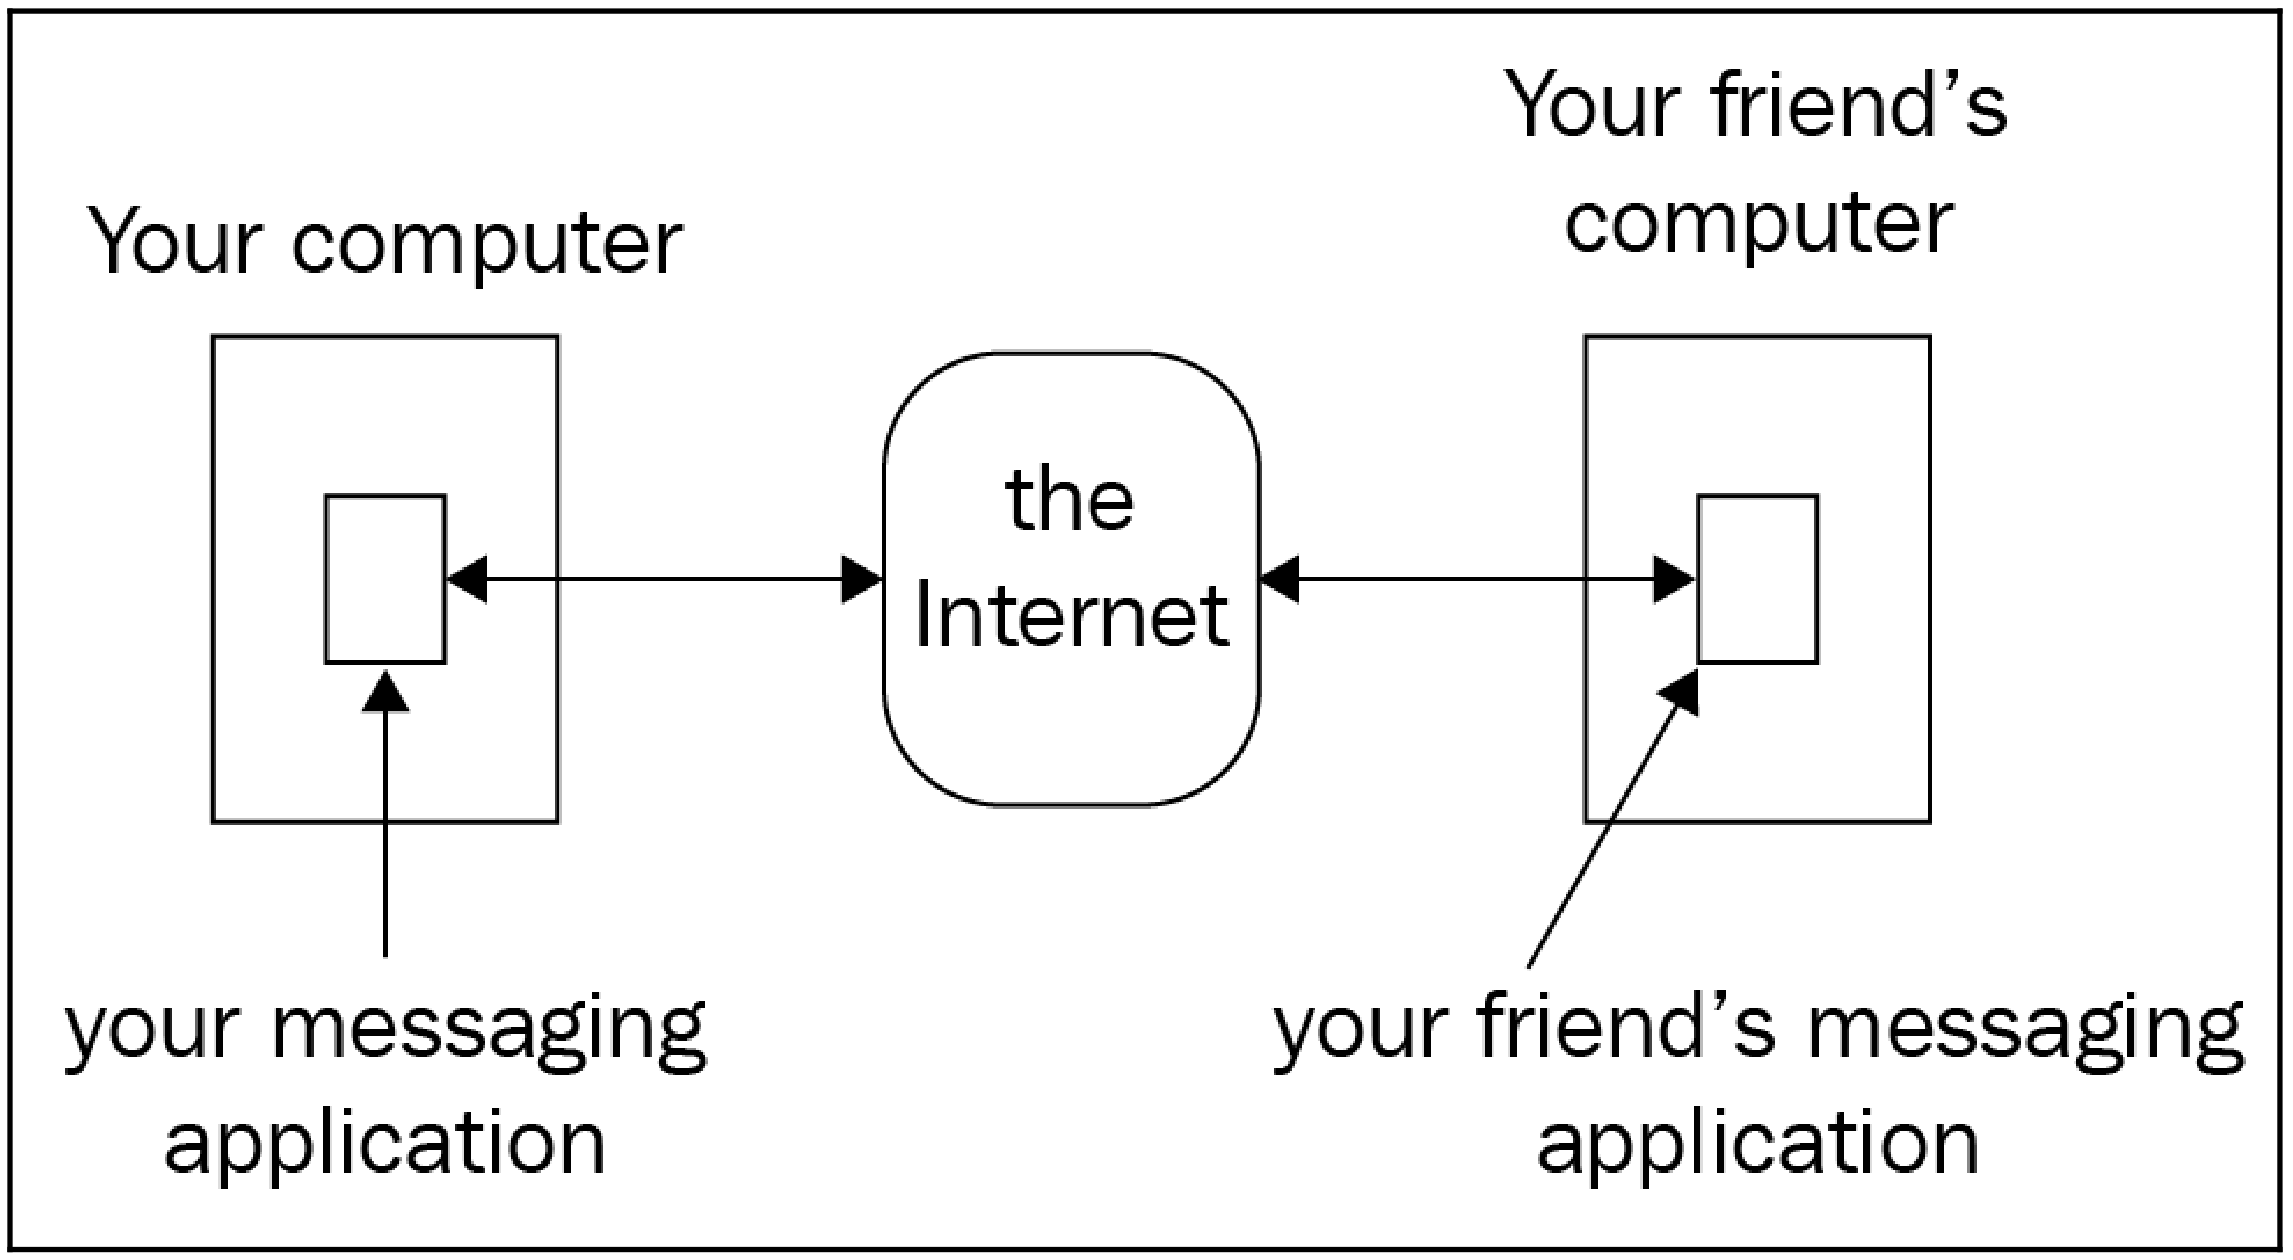
\includegraphics[width=1.0\textwidth]{content/Section-2/Chapter-12/2}
\end{center}

通信的最低层是物理层,它通过媒体传输数据位。在这种情况下,一种媒介就是网线(也可以考虑Wi-Fi通信)。用户应用程序从较底层的网络通信中抽象出来。操作系统提供了程序员所需要的一切。操作系统实现了网络通信的底层细节,比如传输控制协议/Internet协议(TCP/IP)套件。 \par
当应用程序需要访问网络时,无论是局域网还是Internet,都会请求操作系统提供一个接入点。操作系统设法通过使用一个网络适配器和特定的软件与硬件对话来提供一个网络网关。 \par
更详细的说明如下: \par

\begin{center}
	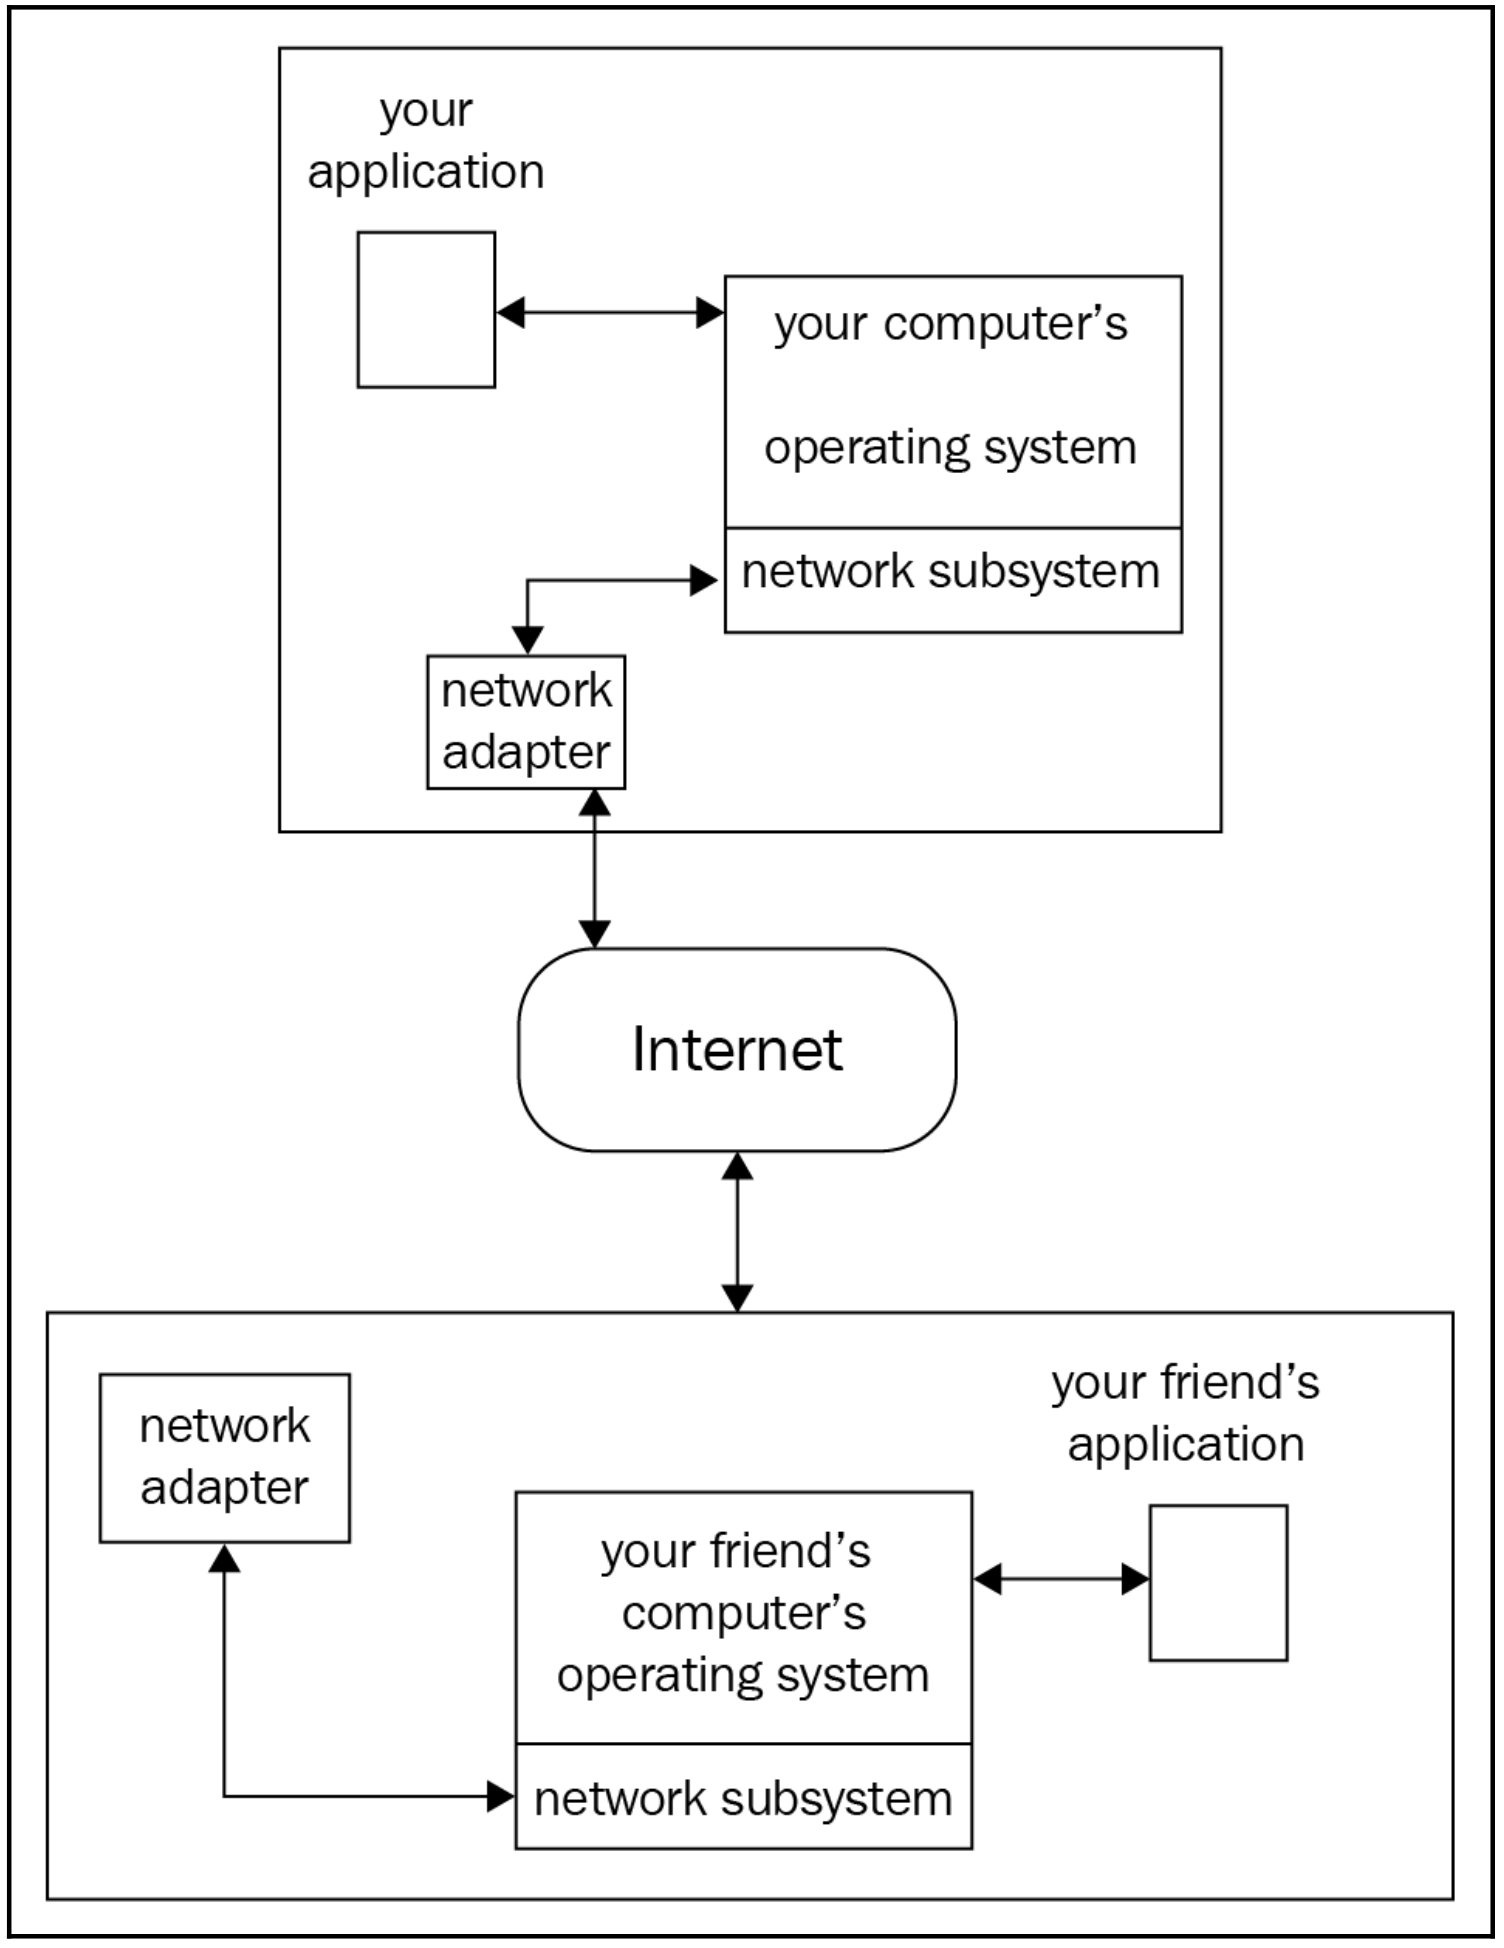
\includegraphics[width=0.6\textwidth]{content/Section-2/Chapter-12/3}
\end{center}

操作系统提供了与其网络子系统一起工作的API。开发者应该关心的主要抽象是套接字。我们可以将套接字视为通过网络适配器发送内容的文件。套接字是通过网络连接两台计算机的接入点,如下图所示: \par

\begin{center}
	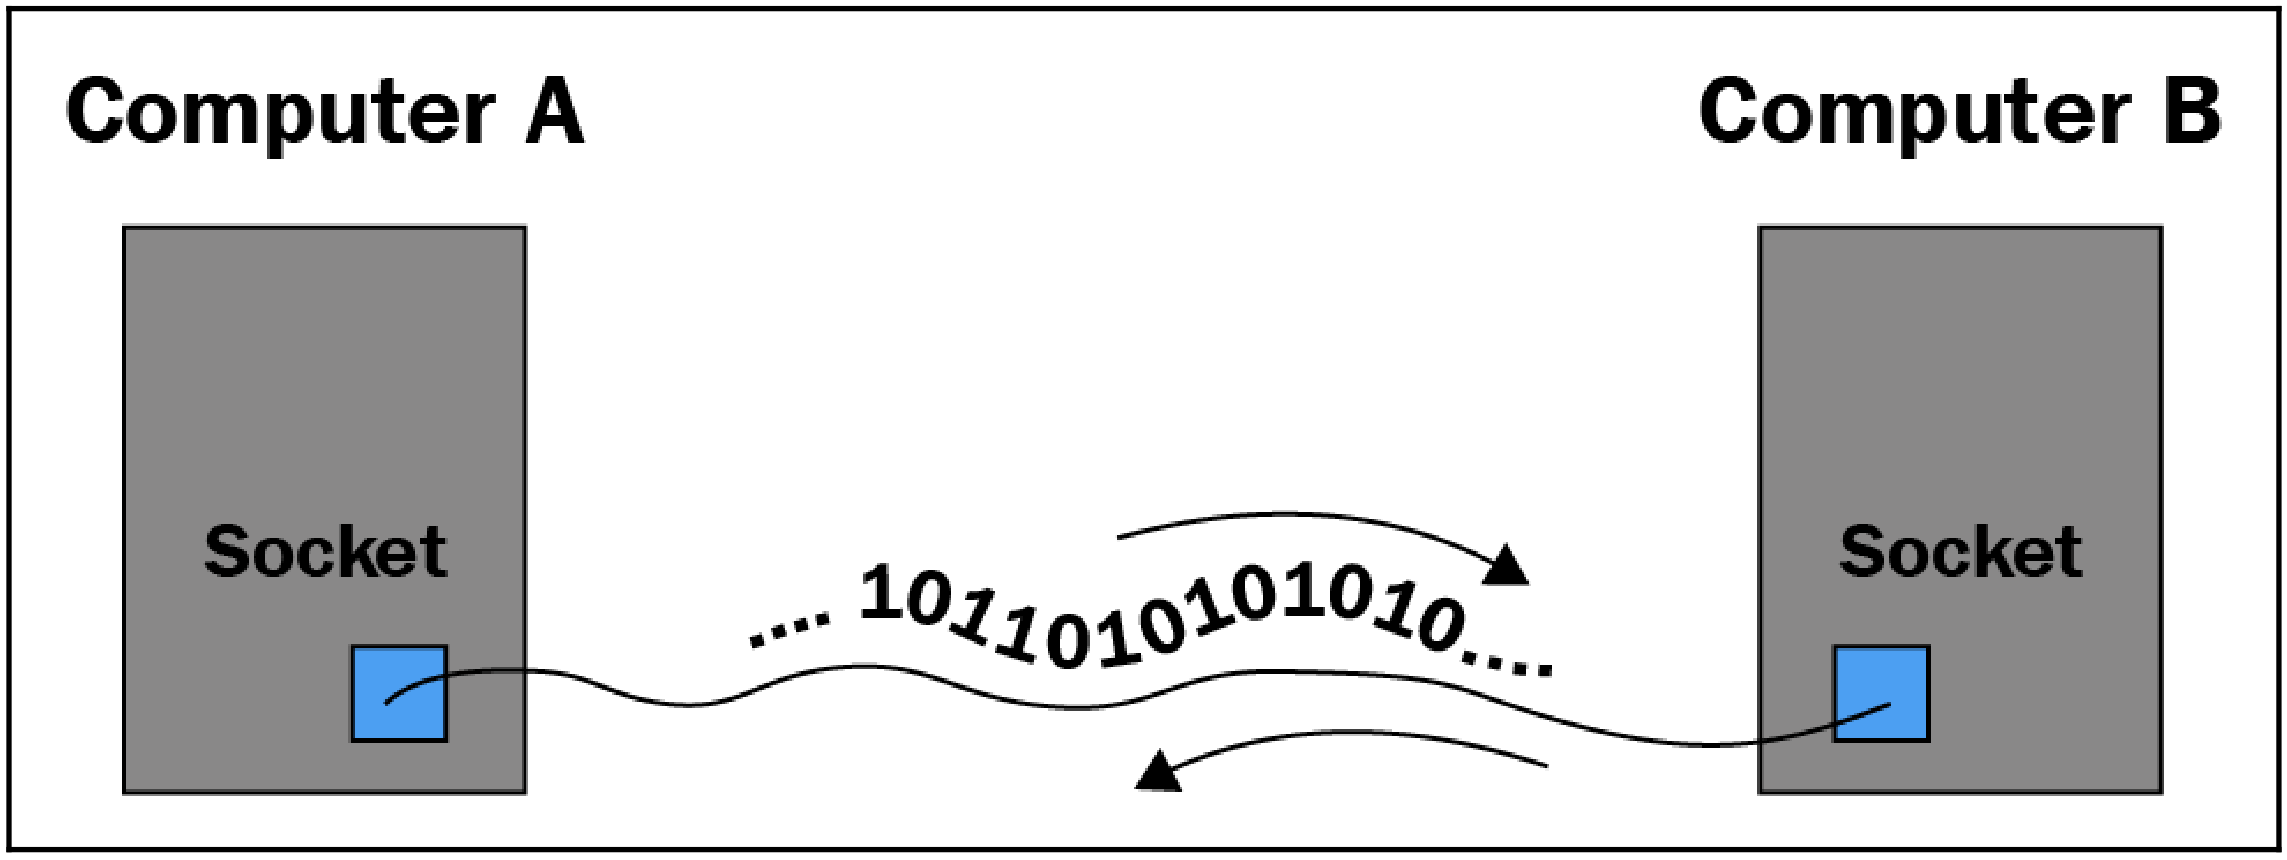
\includegraphics[width=1.0\textwidth]{content/Section-2/Chapter-12/4}
\end{center}

从开发者的角度来看,套接字是一种结构,它允许我们在应用程序中通过网络实现数据。套接字是发送或接收数据的连接点,应用程序通过套接字接收数据。操作系统根据请求为应用程序提供套接字,一个应用程序可以有多个套接字。客户机-服务器体系结构中的客户机应用程序通常使用单个套接字进行操作。现在,让我们详细研究一下套接字编程。 \par

\noindent\textbf{}\ \par
\textbf{使用套接字编写网络应用} \ \par
如前所述,套接字是对网络通信的抽象。我们将它们视为常规文件——所有写入套接字的内容都由操作系统通过网络发送到目的地。所有通过网络接收到的东西都被写进套接字——同样是由操作系统写的。通过这种方式,操作系统为网络应用程序提供了双向通信。 \par
我们假设我们在网络上运行两个不同的应用程序。例如,打开一个Web浏览器,并使用一个消息传递应用程序(如Skype)与朋友聊天。Web浏览器表示客户机-服务器网络体系结构中的客户机应用程序。本例中,服务器是响应请求数据的计算机。例如,在Web浏览器的地址栏中输入一个地址,然后在屏幕上看到生成的Web页面。每当我们访问一个网站时,Web浏览器都会向操作系统请求一个套接字。编码方面,Web浏览器使用操作系统提供的API创建套接字。我们可以用一个更具体的前缀来描述这个套接字:客户端套接字。为了让服务器处理客户端请求,运行Web服务器的计算机必须侦听传入的连接,这时服务器应用创建了一个用于侦听连接的服务器套接字。 \par
只要客户端和服务器之间建立了连接,就可以进行数据通信。下图描述了一个Web浏览器对facebook.com的请求: \par

\begin{center}
	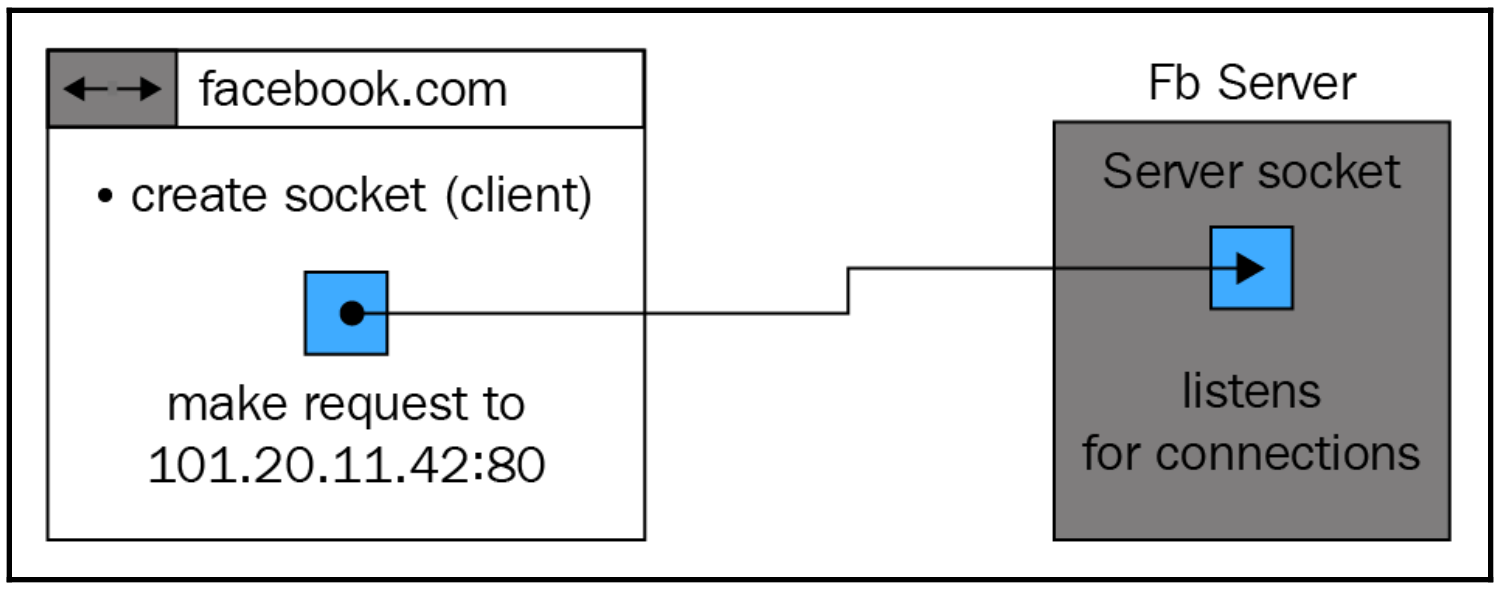
\includegraphics[width=1.0\textwidth]{content/Section-2/Chapter-12/5}
\end{center}

请注意上图中的数字组。这被称为Internet协议(IP)地址。IP地址是我们需要的位置,以便将数据传输到设备。有数十亿的设备连接到互联网上。为了在它们之间做出区分,每个设备都公开一个表示其地址的唯一数值。连接是使用IP协议建立的,我们称它为IP地址。一个IP地址由四组1字节长度的数字组成。它的点分十进制表示形式为X.X.X.X,其中X是1字节数。每个位置的取值范围为0到255。更具体地说,这是一个版本4的IP地址。现代系统使用IPv6地址,它是数字和字母的组合,提供更广泛的可用地址。 \par
创建套接字时,我们将本地计算机的IP地址分配给,我们将套接字绑定到地址。当使用套接字向网络中的另一个设备发送数据时,我们应该设置它的目的地址。目的地址被该设备上的另一个套接字持有。为了在两个设备之间创建连接,我们使用两个套接字。一个合理的问题可能会出现——如果有几个应用程序在设备上运行怎么办?如果我们运行几个应用程序,每个应用程序都为自己创建了一个套接字,那会怎么样?哪一个应该接收传入的数据? \par
要回答这些问题,请仔细看看上面的图表。应该在IP地址的末尾看到冒号后的数字,这称为端口号。端口号是一个由操作系统分配给套接字的2字节长度的数字。由于2字节的长度限制,操作系统不能分配超过65,536个唯一的端口号给套接字,不能有超过65,536个同时运行的进程或线程通过网络进行通信(但是,有一些方法可以重用套接字)。除此之外,还有一些端口号保留给特定的应用程序。这些端口称为知名端口,范围为0 ~ 1023。它们是预留给特权服务的。例如,HTTP服务器的端口号为80。这并不意味着它不能使用其他端口。 \par
我们学习如何在C++中创建套接字。我们将设计一个封装可移植操作系统接口(POSIX)套接字的包装器类,也称为Berkeley或BSD套接字,其有一组用于套接字编程的标准函数。C++的网络编程扩展将是对该语言的巨大补充,草案中包含了网络接口的信息。我们将在本章后面讨论这一点。在此之前,让我们尝试为现有的底层库创建我们自己的网络包装器。当我们使用POSIX套接字时,我们依赖于操作系统的API。操作系统提供了一个API,该API表示用于创建套接字、发送和接收数据等的函数和对象。 \par
POSIX将套接字表示为文件描述符。我们几乎把它当作一个常规文件来使用。文件描述符遵循UNIX哲学,为数据输入/输出提供公共接口。下面的代码会使用socket()函数(定义在<sys/socket.h>头文件中): \par

\begin{lstlisting}[caption={}]
int s = socket(AF_INET, SOCK_STREAM, IPPROTO_TCP);
\end{lstlisting}

socket()函数的声明如下: \par

\begin{lstlisting}[caption={}]
int socket(int domain, int type, int protocol);
\end{lstlisting}

因此,AF\underline{ }INET、SOCK\underline{ }STREAM和IPPROTO\underline{ }TCP都是数值。domain参数指定套接字的协议族。我们使用AF\underline{ }INET来指定IPv4协议。对于IPv6,我们使用AF\underline{ }INET6。第二个参数指定套接字的类型,即它是面向流的套接字还是数据报的套接字。对于每个特定类型,应该相应地指定最后一个参数。在前面的示例中,我们使用IPPROTO\underline{ }TCP指定了SOCK\underline{ }STREAM。传输控制协议(TCP)代表了一个可靠的面向流的协议,这就是我们将类型参数设置为SOCK\underline{ }STREAM的原因。在实现套接字应用之前,让我们了解更多关于网络协议的信息。 \par

\noindent\textbf{}\ \par
\textbf{网络协议} \ \par
网络协议是定义应用程序之间相互通信的规则和数据格式的集合。例如,一个Web浏览器和一个Web服务器通过超文本传输协议(HTTP)进行通信。HTTP更像是一组规则,而不是一个传输协议。传输协议是每一个网络通信的基础。传输协议的一个例子是TCP。我们提到了TCP/IP套件,我们指的是基于IP的TCP实现。我们可以把网络协议(IP)看作是网络通信的核心。 \par
它提供主机到主机的路由和寻址。我们通过互联网发送或接收的所有东西都打包成一个IP包。下面是IPv4数据包的样子: \par

\begin{center}
	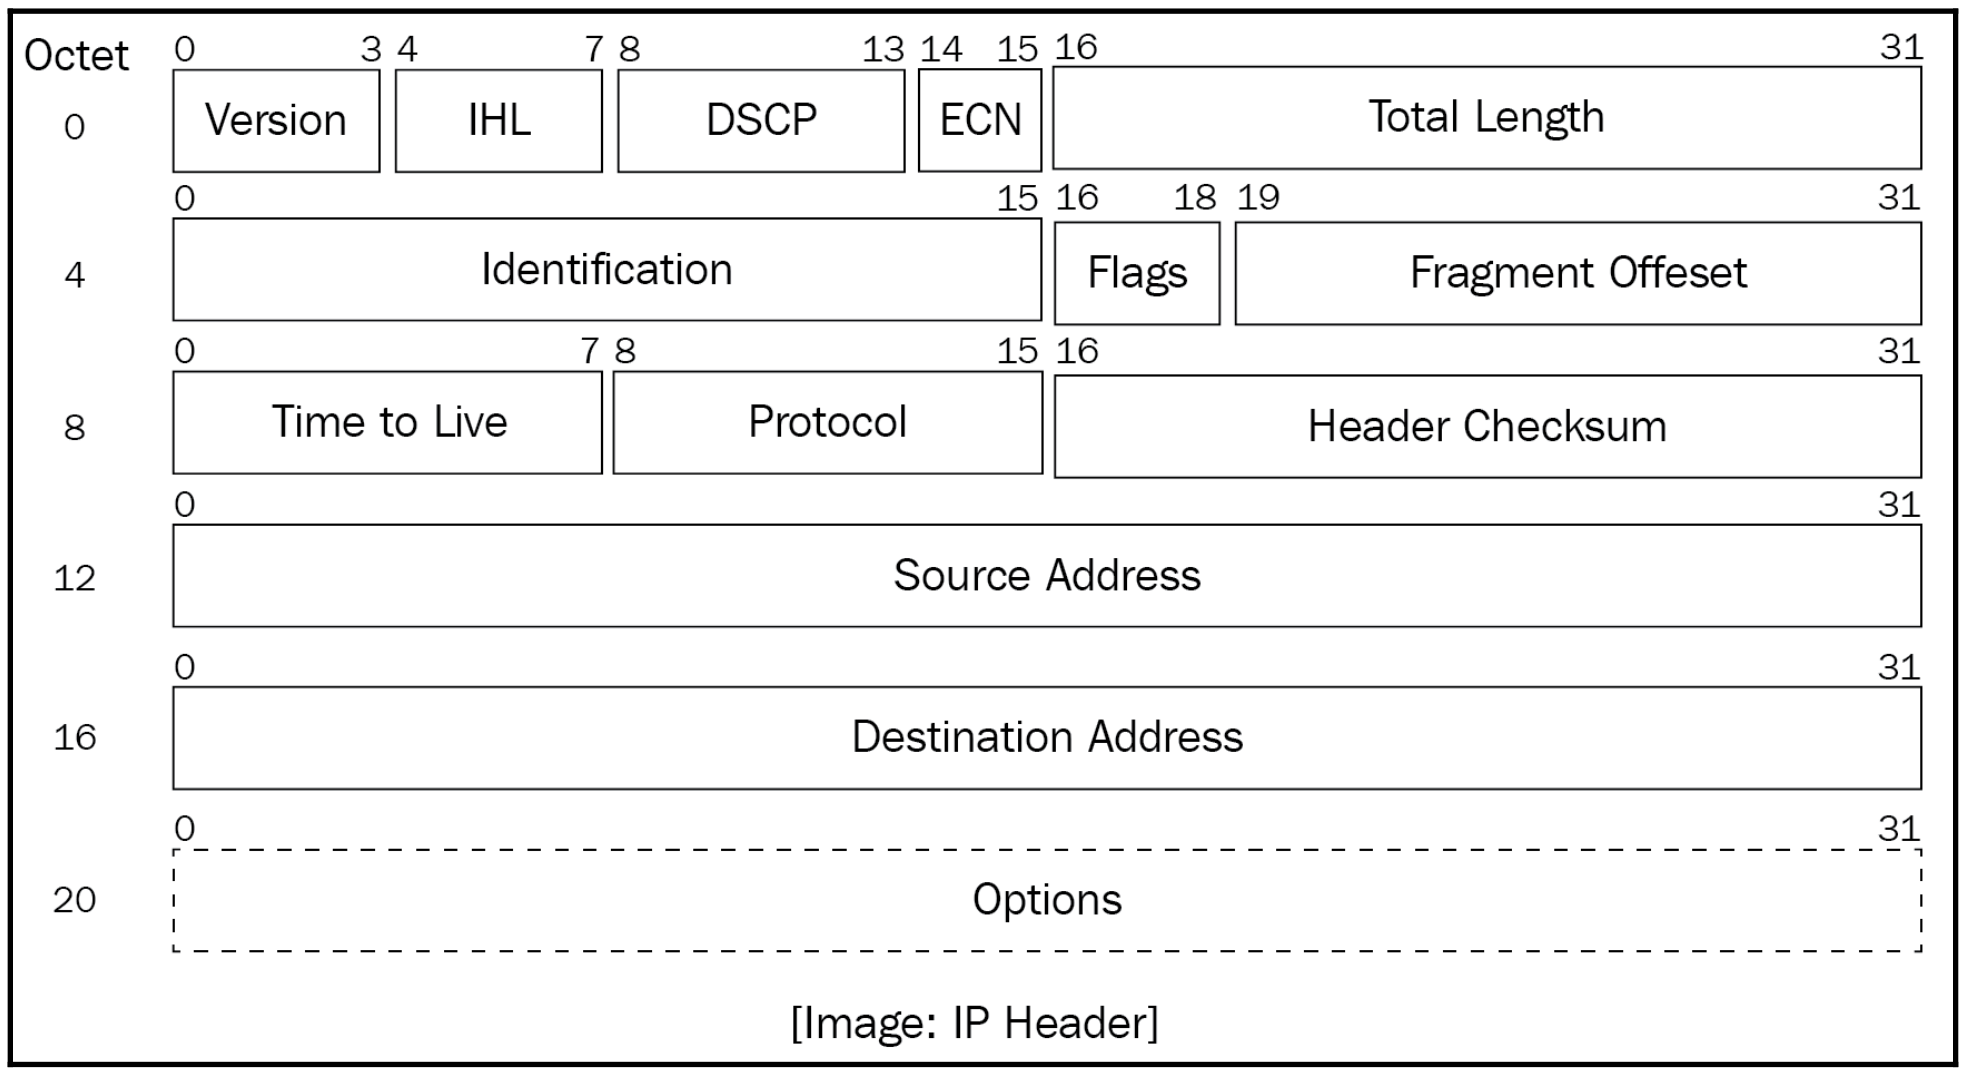
\includegraphics[width=1.0\textwidth]{content/Section-2/Chapter-12/6}
\end{center}

IP报头为20字节,它结合了将包从源地址发送到目的地址所需的标志和选项。在IP协议的域中,我们通常称一个包为数据报。每一层都有其特定的数据包术语。更谨慎的专家讨论将TCP段封装到IP数据报中。把它们叫做包是完全可以的。 \par
更高层次上的每个协议都在通过网络发送和接收的数据上附加元信息,例如:TCP数据封装在IP数据报中。除了这个元信息之外,协议还定义了底层的规则和操作,这些规则和操作应该被执行以完成两个或更多设备之间的数据传输。 \par

\hspace*{\fill} \\ %插入空行

\includegraphics[width=0.05\textwidth]{images/warn}
可以在称为请求注释(Request for Comments, RFC)的特定文档中找到更详细的信息。例如,RFC 791描述了Internet协议,而RFC 793描述了传输控制协议。 \par
\noindent\textbf{}\ \par

许多流行的应用程序——文件传输、电子邮件、Web等等——使用TCP作为它们的主要传输协议。例如,HTTP协议定义了从客户机到服务器传输的消息的格式,反之亦然。实际的传输是使用传输协议进行的——本例中是TCP。然而,HTTP标准并没有将TCP限制为唯一的传输协议。 \par
下图说明了在将TCP报头传递到底层之前,添加了TCP报头: \par

\begin{center}
	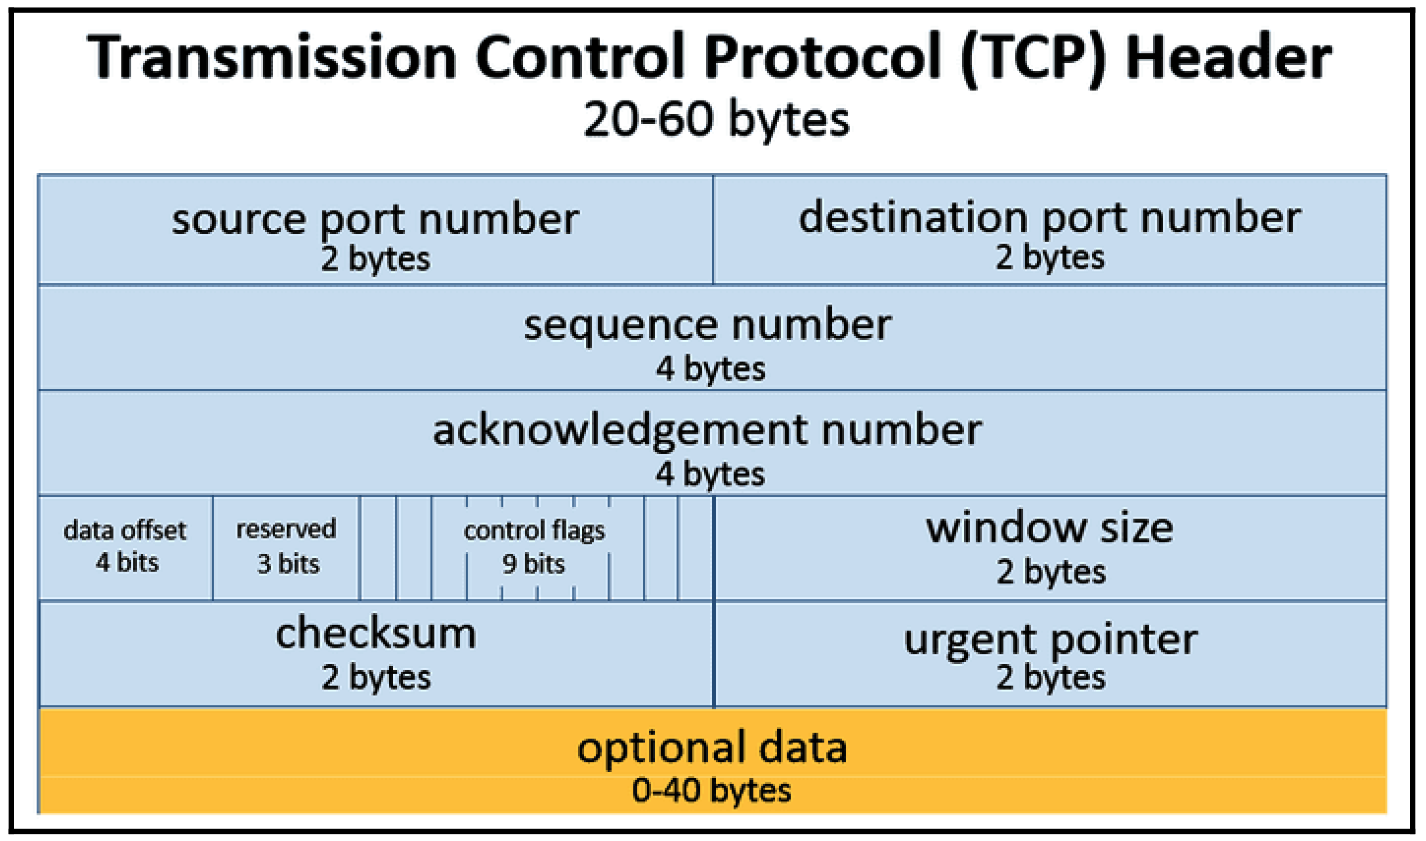
\includegraphics[width=1.0\textwidth]{content/Section-2/Chapter-12/7}
\end{center}

注意源端口号和目的端口号。这些是区分操作系统中运行的进程的唯一标识符。另外,看一下序列和确认号。他们是TCP特定的,并用于传输可靠性。 \par
实际应用中,TCP主要有以下特点: \par

\begin{itemize}
	\item 重新传输丢失的数据
	\item 顺序发送
	\item 数据完整性
	\item 避免拥塞
\end{itemize}

IP(Internet Protocol)不可靠,它不关心丢失的数据包,这就是为什么TCP处理丢失数据包的重传。它用唯一的标识符标记每个包,该标识符应被传输的另一方确认。如果发送方没有收到包的确认码(ACK),协议将重新发送包(有限的次数)。以正确的顺序接收数据包也是至关重要的。TCP重新排序接收到的数据包,以表示正确排序的信息。这就是为什么,当我们在网上听音乐的时候,我们不会在开头听歌曲的结尾。 \par
数据包的重传可能会导致另一个称为网络拥塞的问题。当节点发送数据包的速度不够快时就会发生这种情况。数据包会被卡住一段时间,不必要的重传增加了它们的数量。TCP的各种实现都采用了避免拥塞的算法。 \par
它维护一个阻塞窗口——一个决定可以发送出去的数据量的因素。TCP使用慢启动机制,在初始化连接后缓慢增加拥塞窗口。尽管在相应的请求注释(Request for Comments, RFC)中描述了该协议,但在操作系统中有很多不同的实现机制。 \par
另一个是用户数据报协议(UDP)。与TCP的主要区别是TCP是可靠的。在丢失网络包的情况下,它重新发送相同的包,直到它到达指定的目的地。由于它的可靠性,通过TCP传输数据被认为比使用UDP需要更长的时间。UDP不能保证我们可以正确地传递数据包而不会有损失。相反,开发人员应该注意重新发送、检查和验证数据传输。需要快速通信的应用程序往往依赖UDP。例如,视频电话应用程序或在线游戏使用UDP,因为它的即时性。即使在传输过程中丢失了几个包,也不会影响用户体验。在玩游戏或与朋友视频聊天时出现小故障比等待下一帧游戏或视频好得多。 \par
TCP比UDP慢的一个主要原因是TCP的连接发起过程中有更多的步骤。下图展示了TCP连接建立的过程,也称为三次握手: \par

\begin{center}
	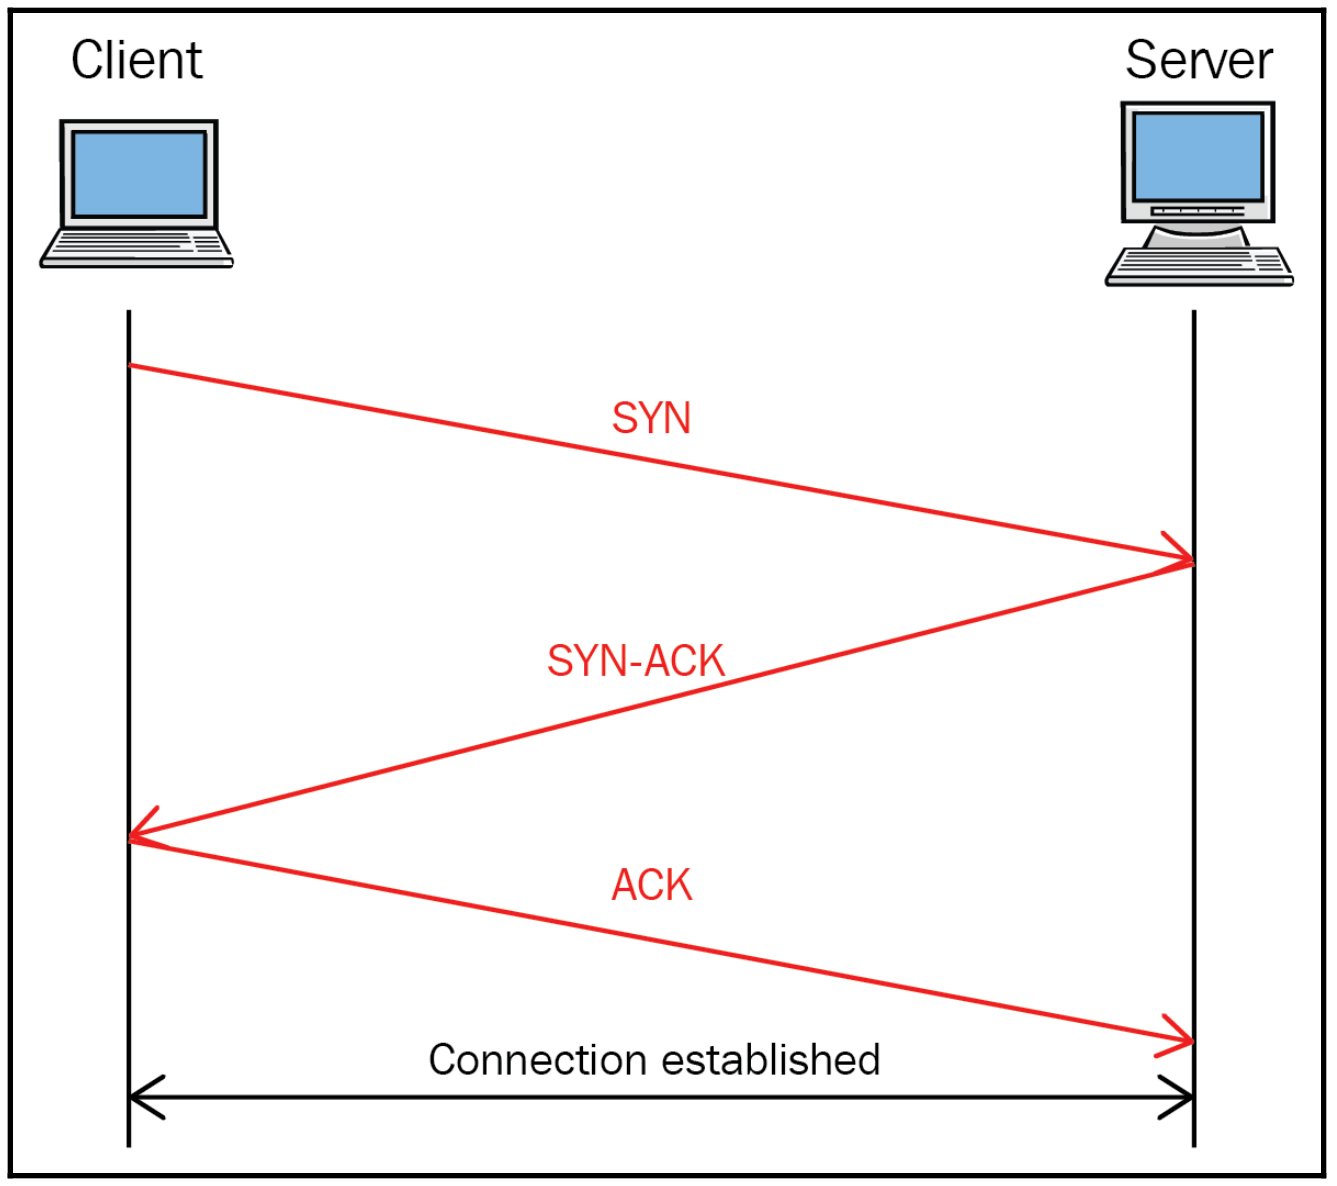
\includegraphics[width=1.0\textwidth]{content/Section-2/Chapter-12/8}
\end{center}

客户端在向服务器发送SYN包时会选择一个随机数。服务器将这个随机数加1,然后选择另一个随机数,然后用一个SYN-ACK报文进行应答。客户机将从服务器接收到的两个数字都加1,并通过向服务器发送最后一个ACK来完成握手。三次握手成功完成后,客户端和服务器就可以相互传输数据包了。这个连接建立过程适用于每一个TCP连接。对网络应用程序的开发人员隐藏了握手的细节。我们创建套接字并开始侦听传入的连接。 \par
请注意这两种端点之间的区别。其中一个是客户。在实现网络应用程序时,我们应该明确区分客户端和服务器,因为它们有不同的实现。这也与套接字类型有关。当创建一个服务器套接字时,我们让它监听传入的连接,而客户端不监听——发出请求。下图描述了客户端和服务器的某些函数及其调用顺序: \par

\begin{center}
	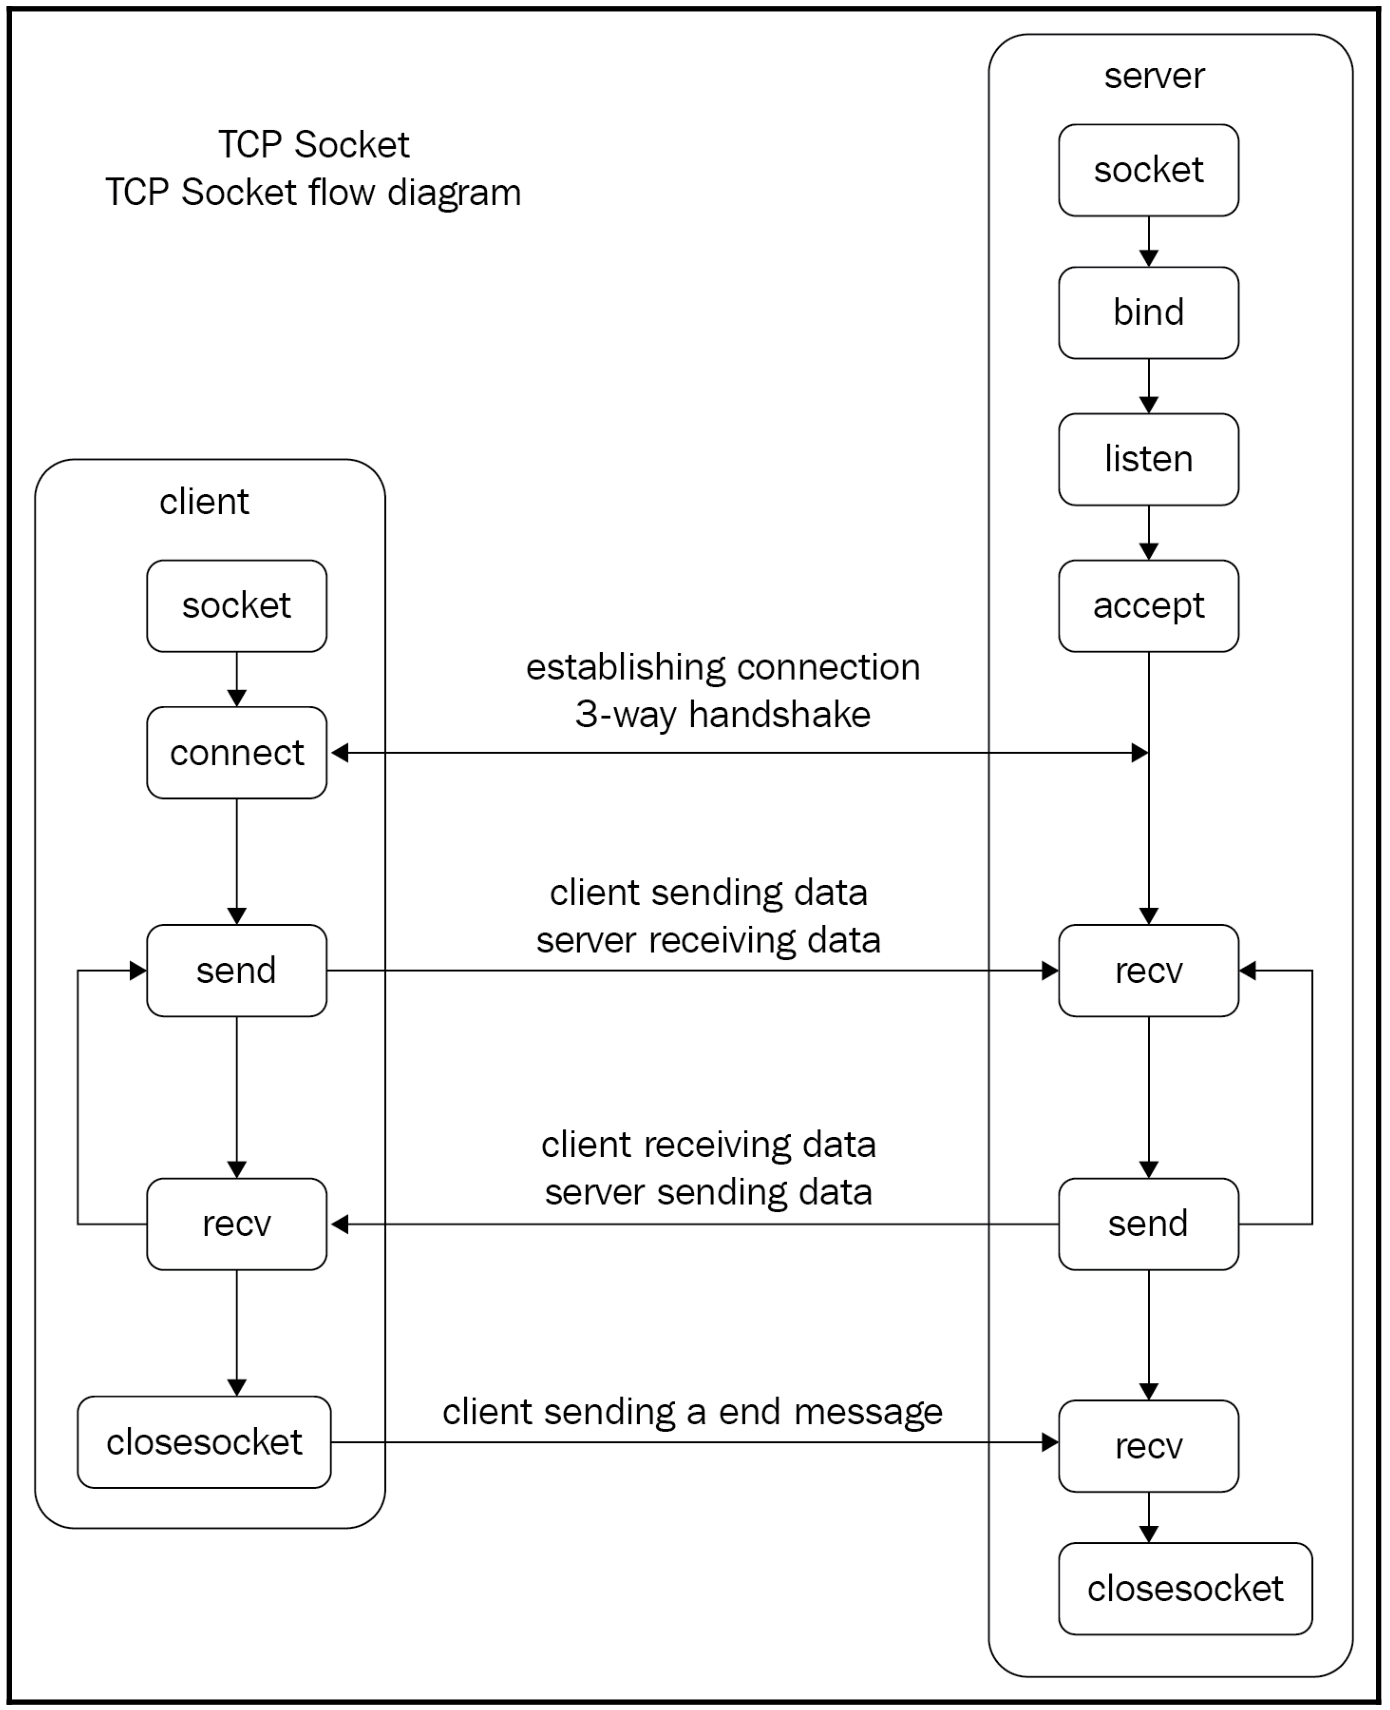
\includegraphics[width=1.0\textwidth]{content/Section-2/Chapter-12/9}
\end{center}

在代码中创建套接字时,我们指定套接字的协议和类型。当我们想要在两个端点之间建立可靠的连接时,我们选择TCP。有趣的是,我们可以使用TCP这样的传输协议来构建我们自己的协议。假设我们定义了要发送和接收的特殊文档格式,以便有效地处理通信。例如,每个文档都应该以单词pack开头。HTTP以同样的方式工作。它使用TCP进行传输,并在其上定义一种通信格式。在UDP的情况下,我们还应该设计并实现一个通信的可靠性策略。上面的图显示了TCP如何在两个端点之间建立连接。客户机向服务器发送SYN请求。服务器用SYN-ACK响应进行应答,让客户机知道可以继续握手。最后,客户机用一个ACK应答服务器,声明连接正式建立。他们可以随时交流。 \par

\hspace*{\fill} \\ %插入空行

\includegraphics[width=0.05\textwidth]{images/tip}
同步(SYN)和ACK是协议定义的术语,在网络编程中很常见。 \par
\noindent\textbf{}\ \par

UDP不以这种方式工作。它将数据发送到目的地,而不必担心已建立的连接。如果你使用UDP,但需要一些可靠性,你应该自己实现它,例如:通过检查数据的一部分是否到达目的地,可以用一个自定义的ACK包等待目的地的应答检查它。大多数面向可靠性的实现可能重复已经存在的协议,比如TCP。然而,在许多情况下,您并不需要它们,例如:不需要避免拥塞,因为不需要发送相同的数据包两次。 \par
在前一章我们设计了一款策略游戏。假设这是一款在线游戏,你正在与一个真正的对手对战,而不是一个自动的敌人玩家一起游戏。游戏的每一帧都是基于网络接收到的数据进行渲染的。如果我们努力确保数据传输的可靠性,增加数据的完整性,并确保没有数据包丢失,用户体验可能会因为玩家的不同步而受到损害,这个场景很适合使用UDP。我们可以在不使用重传策略的情况下实现数据传输,从而保证游戏的速度。当然,使用UDP并不会缺少可靠性。在相同的场景中,我们可能需要确保数据包被玩家成功接收。例如,当玩家投降时,我们应该确保对手收到消息。因此,我们可以根据数据包优先级有条件的可靠性。UDP在网络应用中提供了非常高灵活性和速度。 \par
让我们看一下TCP服务器应用程序的实现。 \par

\noindent\textbf{}\ \par
\textbf{设计一个网络应用} \ \par
设计带有需要网络连接的子系统的应用程序的方法,与完全与网络相关的应用程序不同。后者的一个例子可能是用于文件存储和同步的客户机-服务器应用程序(如Dropbox)。它由服务器和客户端组成,其中客户端作为桌面或移动应用程序安装,也可以用作文件资源管理器。Dropbox控制的系统中文件的每次更新都将立即与服务器同步。这样,文件就会一直保存在云端,只要有网络连接,你就可以在任何地方访问它们。 \par
我们将为文件存储和操作设计一个类似的简化服务器应用程序。服务器的主要任务如下: \par

\begin{itemize}
	\item 从客户端应用程序接收文件
	\item 将文件存储在指定的位置
	\item 客户端请求时发送文件
\end{itemize}

参考第10章,我们可以进一步了解应用程序的顶层设计: \par

\begin{center}
	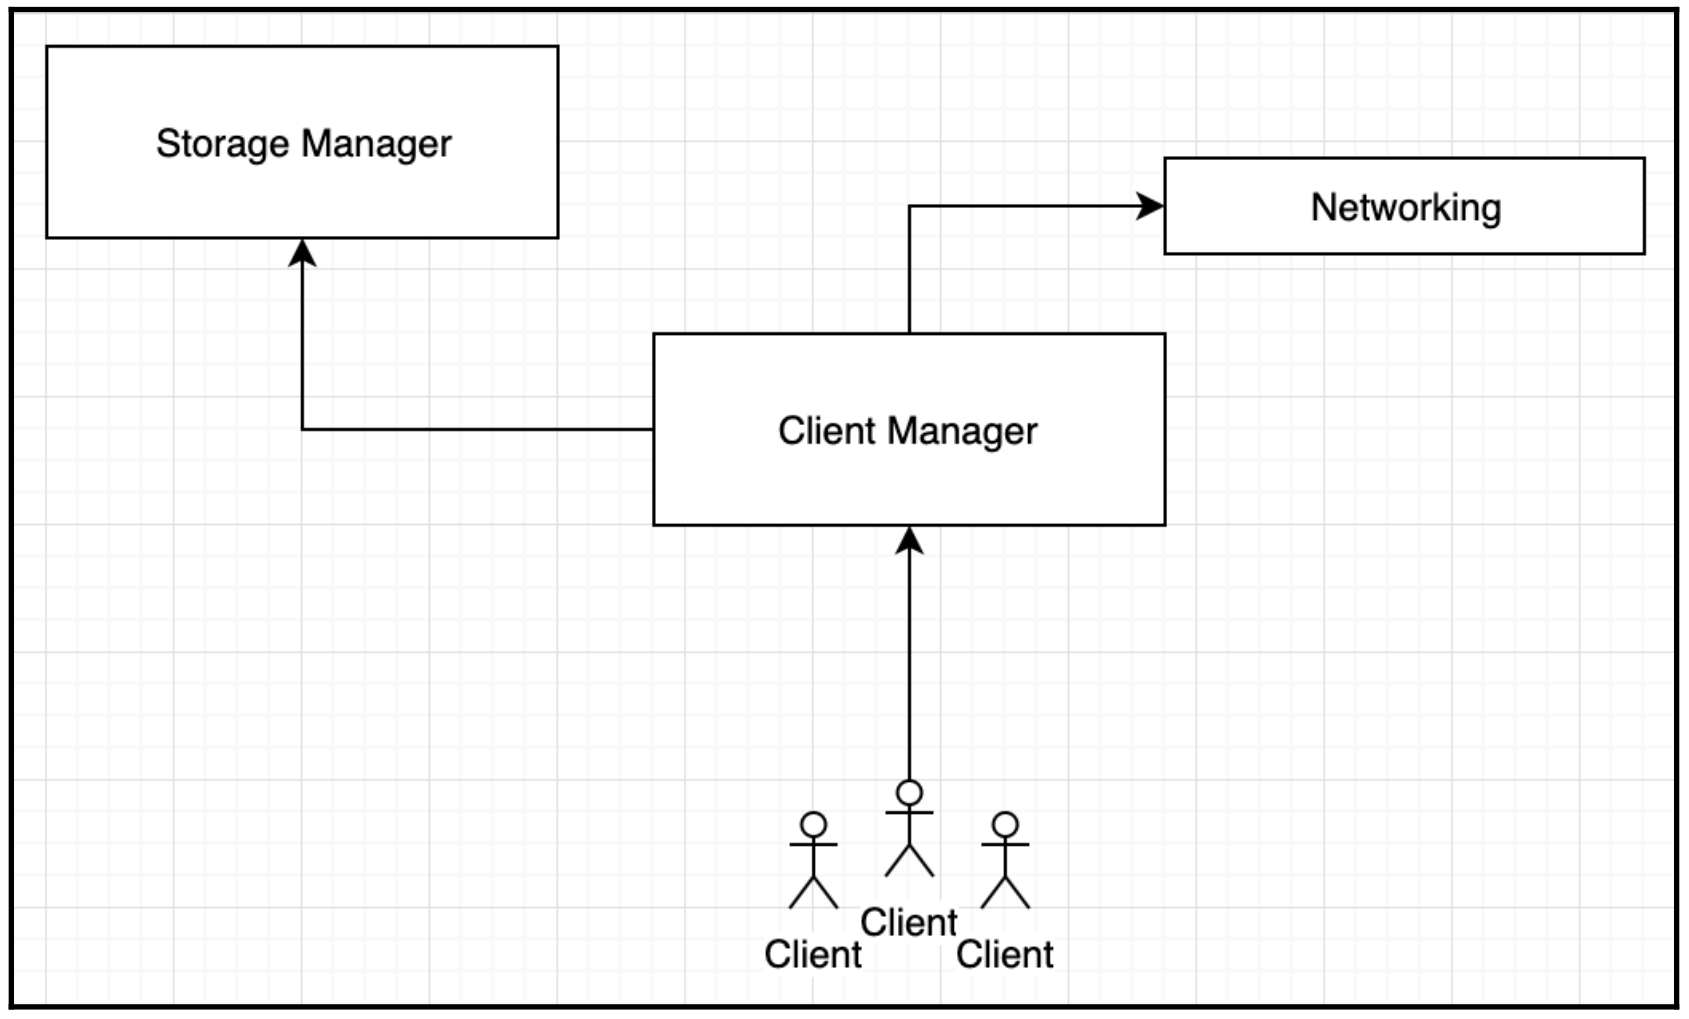
\includegraphics[width=1.0\textwidth]{content/Section-2/Chapter-12/10}
\end{center}

上图中的每个矩形表示一个类或与特定任务相关的类的集合。例如,存储管理器处理与存储和检索文件相关的一切。在这一点上,是否使用诸如文件、位置、数据库等类我们并不太担心。 \par
客户端管理器是一个或一组类,表示处理与客户端身份验证或授权(通过客户端,我们指的是客户端应用程序)、与客户端保持稳定连接、从客户端接收文件、向客户端发送文件等等相关的一切。 \par
在本章中,我们特别强调了网络是一个值得关注的实体。所有与网络连接相关的事情,以及与客户机之间的数据传输,都是通过网络来处理的。现在,让我们看看可以使用哪些功能来设计Networking类(为了方便起见,我们将其称为Network Manager)。 \par

\noindent\textbf{}\ \par
\textbf{使用POSIX套接字} \ \par
如前所述,socket()、bind()和accept()等函数是大多数Unix系统默认支持的库函数,包含在<sys/socket.h>头文件中。除此之外,我们还需要其他几个头文件。让我们实现经典的TCP服务器示例,并将其封装在文件传输应用程序服务器的网络模块中。 \par
正如我们前面提到的,服务器端开发在套接字类型及其行为方面不同于客户端开发。尽管双方都使用套接字操作,但服务器端套接字一直在监听传入的连接,而客户端套接字则发起与服务器的连接。为了让服务器套接字等待连接,我们创建了一个套接字,并将其绑定到客户机将尝试连接到的服务器IP地址和端口号。下面的C代码表示TCP服务器套接字的创建和绑定: \par

\begin{lstlisting}[caption={}]
int s = socket(AF_INET, SOCK_STREAM, 0);

struct sockaddr_in server;
server.sin_family = AF_INET;
server.sin_port = htons(port);
server.sin_addr.s_addr = INADDR_ANY;

bind(s, (struct sockaddr*)&server, sizeof(server));
\end{lstlisting}

第一个调用创建一个套接字。第三个参数设置为0,表示将根据套接字的类型选择默认协议。类型作为第二个参数SOCK\underline{ }STREAM传递,它使协议值在默认情况下等于IPPROTO\underline{ }TCP。函数的作用是:将套接字与指定的IP地址和端口号绑定。我们在sockaddr\underline{ }in结构中指定了它们,该结构将网络地址相关的细节组合在了其中。 \par

\hspace*{\fill} \\ %插入空行

\includegraphics[width=0.05\textwidth]{images/warn}
尽管我们在前面的代码中跳过了这一点,但应该考虑检查对socket()和bind()函数(以及POSIX套接字中的其他函数)的调用,防止出现错误。在出现错误的情况下,它们都返回-1。 \par
\noindent\textbf{}\ \par

另外,请注意htons()函数。它负责将其参数转换为网络字节顺序,这个问题隐藏在计算机的设计方式中。一些机器(例如:英特尔处理器)使用小端字节顺序,而另一些则使用大端顺序。小端顺序将最低有效字节放在前面。大端顺序将最有效字节放在前面。下图显示了两者之间的区别: \par

\begin{center}
	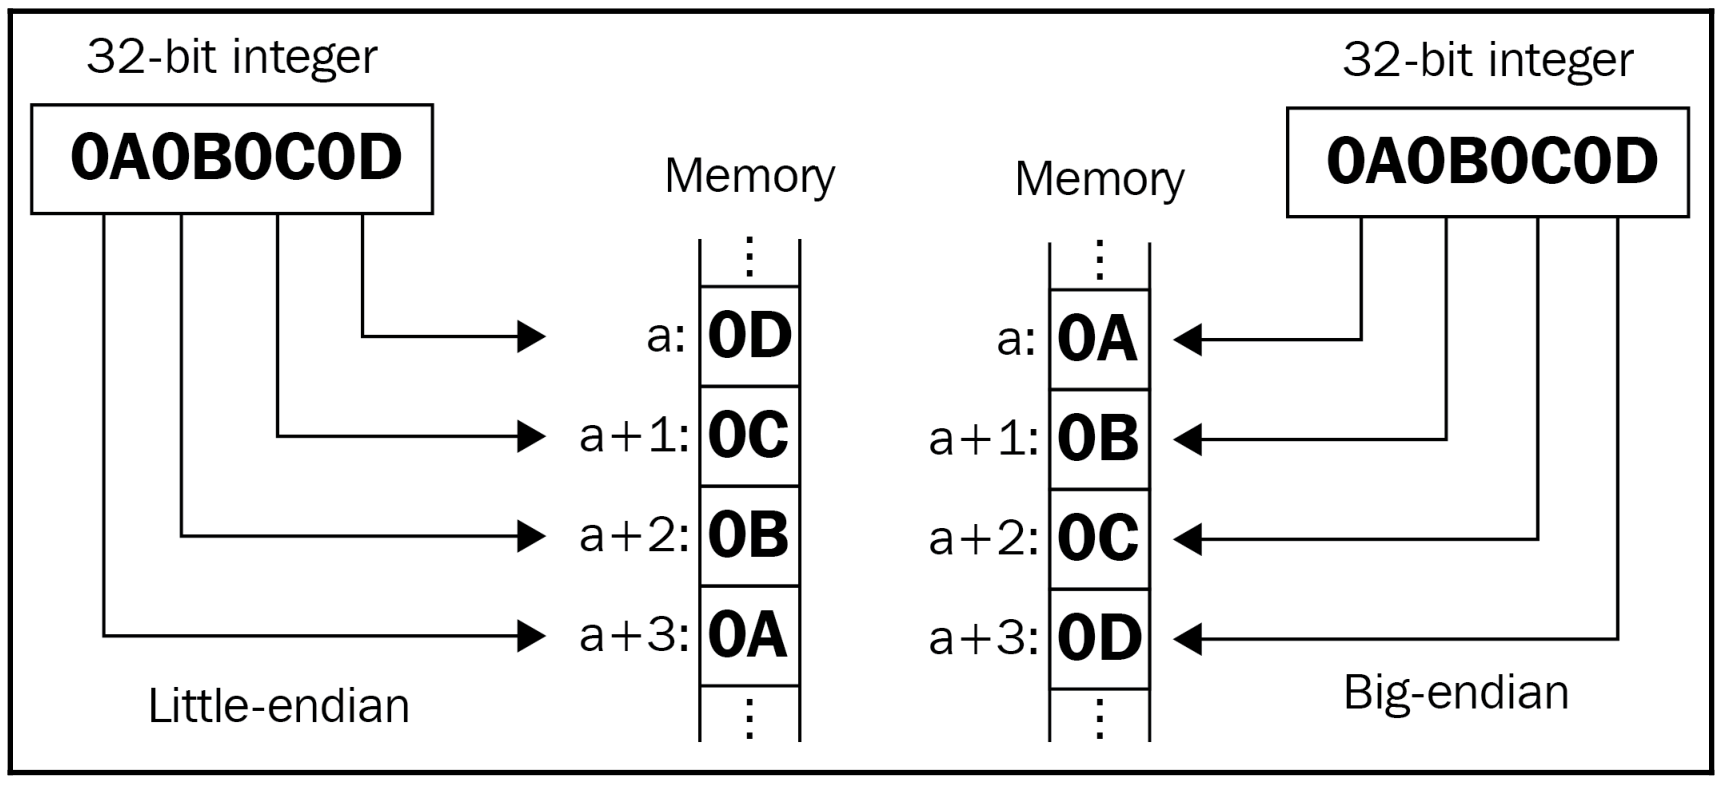
\includegraphics[width=1.0\textwidth]{content/Section-2/Chapter-12/11}
\end{center}

网络字节顺序是独立于特定机器架构的一种约定。函数的作用是:将提供的端口号从主机字节顺序(小端或大端)转换为网络字节顺序(独立于机器)。 \par
就这样,套接字就准备好了。现在,我们应该指定它为传入连接做好准备。为此,我们使用listen()函数: \par

\begin{lstlisting}[caption={}]
listen(s, 5);
\end{lstlisting}

顾名思义,它监听传入的连接。传递给listen()函数的第二个参数指定服务器在丢弃新的传入请求之前将排队的连接数。在前面的代码中,我们指定5为最大值。在高负载环境中,我们将增加这个数字。最大数量由<sys/socket.h>头文件中定义的SOMAXCONN常量指定。 \par
选择待办数量(listen()函数的第二个参数)的选择基于以下因素: \par

\begin{itemize}
	\item 如果连接请求的速率在短时间内很高,则待办数应该有一个较大的值。
	\item 服务器处理传入连接的持续时间。时间越短,待办数就越小。
\end{itemize}

当连接初始化发生时,我们可以放弃它,也可以接受它并继续处理连接。这就是为什么我们在下面的代码片段中使用了accept()函数的原因: \par

\begin{lstlisting}[caption={}]
struct sockaddr_in client;
int addrlen;
int new_socket = accept(s, (struct sockaddr_in*)&client, &addrlen);
// use the new_socket
\end{lstlisting}

在上述代码中需要考虑的两件事如下: \par

\begin{itemize}
	\item 首先,接受的套接字连接信息写入客户机的sockaddr\underline{ }in结构体中。我们可以从这个结构中收集关于客户机的一切必要信息。
	\item 接下来,注意accept()函数的返回值。它是一个新的套接字,用于处理来自特定客户端的请求。下一个对accept()函数的调用将返回另一个值,该值将代表另一个具有单独连接的客户端。我们应该正确地处理这个问题,因为accept()调用正在阻塞,并等待新的连接请求。我们将修改前面的代码,以便它接受在单独的线程中处理的多个连接。
\end{itemize}

前面代码中带有注释的最后一行声明,可以使用new\underline{ }socket接收或向客户机发送数据。让我们看看如何实现这一点,然后开始设计我们的Networking类。要读取套接字接收到的数据,我们需要使用recv()函数,如下所示: \par

\begin{lstlisting}[caption={}]
char buffer[BUFFER_MAX_SIZE]; // define BUFFER_MAX_SIZE based on the
specifics of the server
recv(new_socket, buffer, sizeof(buffer), 0);
// now the buffer contains received data
\end{lstlisting}

recv()函数接受一个char*缓冲区,以便将数据写入其中。在sizeof(buffer)时停止写入。函数的最后一个参数是我们可以为读取设置的附加标志,应该考虑多次调用该函数来读取大于BUFFER\underline{ }MAX\underline{ }SIZE的数据。 \par
最后,为了通过套接字发送数据,调用send()函数,如下所示: \par

\begin{lstlisting}[caption={}]
char msg[] = "From server with love";
send(new_socket, msg, sizeof(msg), 0);
\end{lstlisting}

至此,我们已经介绍了实现服务器应用程序所需的几乎所有函数。现在,让我们将它们封装在一个C++类中,并结合多线程,就可以并发地处理客户机的请求了。 \par

\noindent\textbf{}\ \par
\textbf{实现POSIX套接字包装类} \ \par
让我们设计并实现一个类,它将作为基于网络的应用程序的起点。类的主接口如下所示: \par

\begin{lstlisting}[caption={}]
class Networking
{
public:
	void start_server();
	
public:
	std::shared_ptr<Networking> get_instance();
	void remove_instance();
	
private:
	Networking();
	~Networking();
	
private:
	int socket_;
	sockaddr_in server_;
	std::vector<sockaddr_in> clients_;
	
private:
	static std::shared_ptr<Networking> instance_ = nullptr;
	static int MAX_QUEUED_CONNECTIONS = 1;
};
\end{lstlisting}

Networking类很自然地成为单例,因为想要单个实例来侦听传入的连接。拥有多个对象也很重要,每个对象代理与客户机的单独连接。让我们逐步完善类设计。我们看到,每个新的客户端套接字是在服务器套接字侦听,并接受连接请求之后创建的。 \par
之后,我们可以通过新的客户端套接字发送或接收数据。服务器的运行方式与下图类似: \par

\begin{center}
	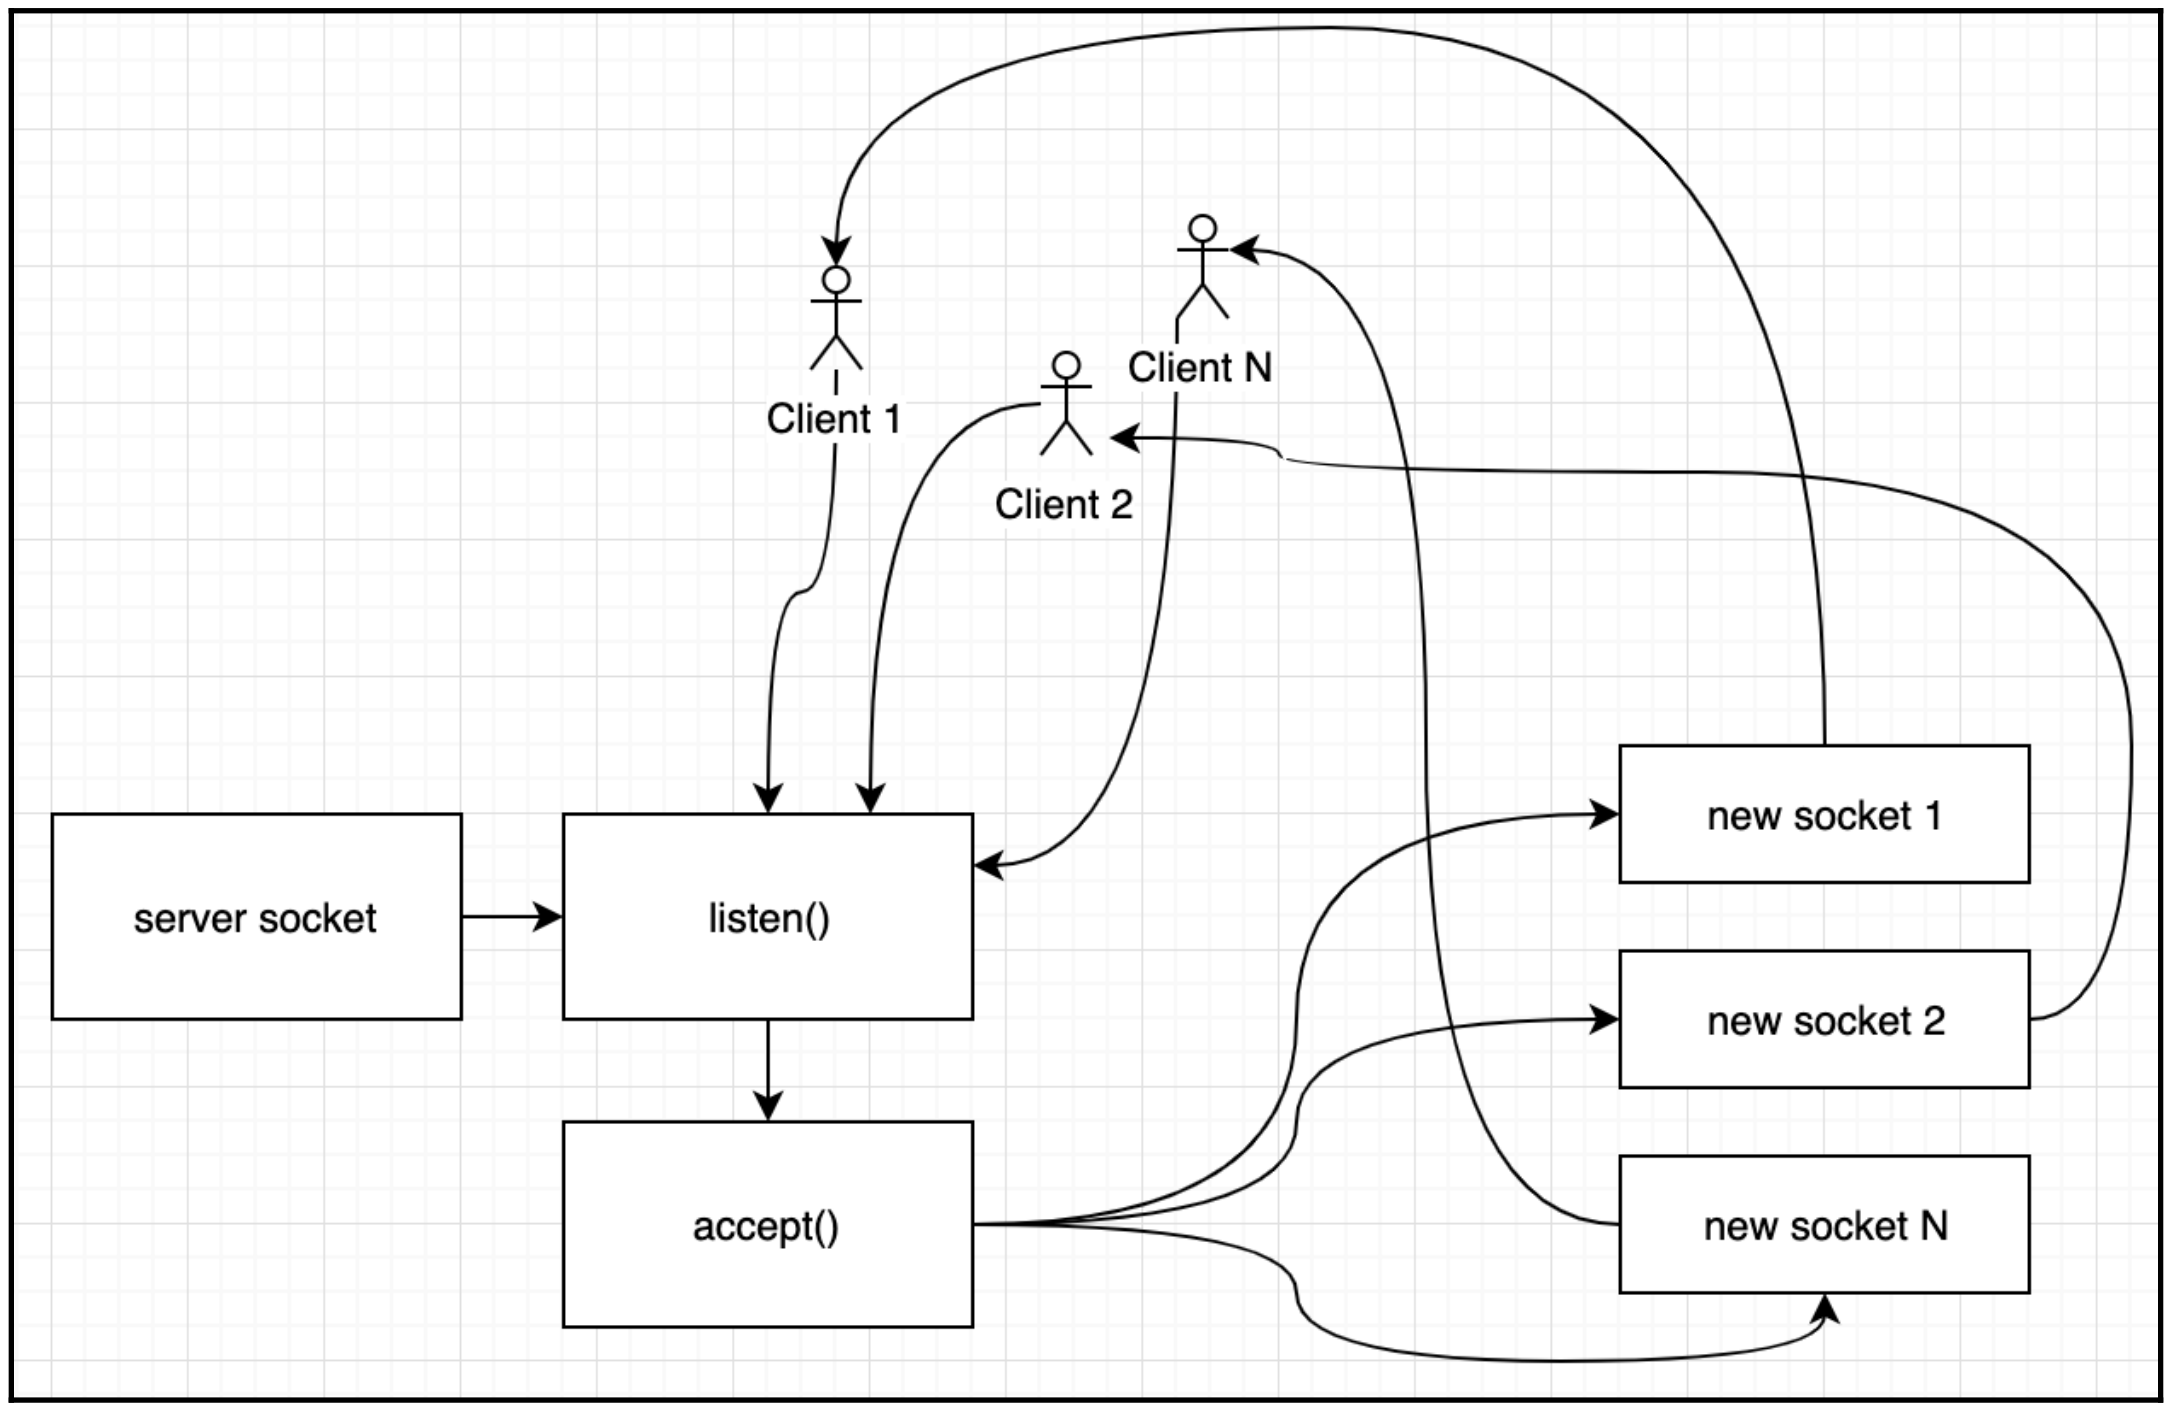
\includegraphics[width=1.0\textwidth]{content/Section-2/Chapter-12/12}
\end{center}

也就是说,在接受每个传入连接之后,我们将为连接提供单独的套接字,并将它们存储在网络类的clients\underline{}中。因此,可以在并发函数中编写创建服务器套接字、侦听和接受新连接的主要逻辑。start\underline{}server()函数作为服务器侦听传入连接的起点。下面的代码块说明了这一点: \par

\begin{lstlisting}[caption={}]
void Networking::start_server()
{
	socket_ = socket(AF_INET, SOCK_STREAM, 0);
	// the following check is the only one in this code snippet
	// we skipped checking results of other functions for brevity,
	// you shouldn't omit them in your code
	if (socket_ < 0) {
		throw std::exception("Cannot create a socket");
	}
	struct sockaddr_in server;
	server.sin_family = AF_INET;
	server.sin_port = htons(port);
	server.sin_addr.s_addr = INADDR_ANY;
	
	bind(s, (struct sockaddr*)&server, sizeof(server));
	listen(s, MAX_QUEUED_CONNECTIONS);
	// the accept() should be here
}
\end{lstlisting}

现在,我们已经在应该接受传入连接的地方停止了(请参阅前面代码片段中的注释)。这里我们有两个选择(实际上不止两个选择,但我们只讨论其中的两个)。我们可以直接在start\underline{ }server()函数中调用accept(),也可以实现一个单独的函数,Networking类用户可以随时调用这个函数。 \par

\hspace*{\fill} \\ %插入空行

\includegraphics[width=0.05\textwidth]{images/tip}
对于项目中的每个错误情况都有特定的异常类,这不是一个坏习惯。在考虑自定义异常时,可能会重写上述代码。你们可以把它作为作业来做。 \par
\noindent\textbf{}\ \par

其中一个选项是start\underline{ }server()函数中的accept()函数,它将每个新连接推入clients\underline{ },如下所示: \par

\begin{lstlisting}[caption={}]
void Networking::start_server()
{
	// code omitted for brevity (see in the previous snippet)
	while (true) {
		sockaddr_in client;
		int addrlen;
		int new_socket = accept(socket_, (sockaddr_in*)&client, &addrlen);
		clients_.push_back(client);
	}
}
\end{lstlisting}

我们用了无限循环。这听起来可能很糟糕,但是只要服务器在运行,就必须接受新的连接。然而,我们都知道无限循环会阻塞代码的执行,它永远不会离开start\underline{ }server()函数。我们介绍的网络应用程序是至少包含三个组件的项目:客户端管理器、存储管理器和我们正在设计的Networking类。 \par
一个组件的执行不得对其他组件产生不良影响,我们可以使用线程让一些组件在后台运行。运行在线程上下文中的start\underline{ }server()函数是一个很好的解决方案,但现在应该关注在第8章中讨论的同步问题。 \par
此外,还要注意前面循环的不完整性。在接受连接后,它将客户端数据推入clients\underline{ }。我们应该考虑使用另一种结构,因为我们还需要存储套接字描述符和客户机。我们可以使用std::undordered\underline{ }map将套接字描述符映射到客户端连接信息,使用简单的std::pair或std::tuple也可以。 \par
让我们更进一步,创建一个表示客户端连接的自定义对象,如下所示: \par

\begin{lstlisting}[caption={}]
class Client
{
public:
	// public accessors
	
private:
	int socket_;
	sockaddr_in connection_info_;
};
\end{lstlisting}

我们修改Networking类,使其存储一个客户端对象的vector: \par

\begin{lstlisting}[caption={}]
std::vector<Client> clients_;
\end{lstlisting}

现在,我们可以改变设计方法,让客户端对象负责发送和接收数据: \par

\begin{lstlisting}[caption={}]
class Client
{
public:
	void send(const std::string& data) {
		// wraps the call to POSIX send()
	}

	std::string receive() {
		// wraps the call to POSIX recv()
	}

	// code omitted for brevity
};
\end{lstlisting}

我们可以将一个std::thread对象附加到Client类,以便每个对象在单独的线程中处理数据传输。但应该注意不要让系统饥饿。传入连接的数量可能会急剧增加,服务器应用程序将会卡住。我们将在下一节讨论安全问题时讨论这个场景。建议利用线程池,既可以帮助我们重用线程,又可以控制程序中运行的线程数量。 \par
类的最终设计取决于我们接收和发送给客户机的数据类型。至少有两种不同的方法。其中一个是连接到客户端,接收必要的数据,然后关闭连接。第二种方法是实现客户机和服务器通信的协议。尽管它听起来很复杂,但协议可能很简单。 \par
它还具有可扩展性,并使应用程序更加健壮,因为随着项目的发展,可以支持更多的特性。下一节中,当我们讨论如何保护网络服务器应用程序时,我们将回到设计用于对客户机请求进行身份验证的协议。 \par

\noindent\textbf{}\ \par
\textbf{使用C++代码} \ \par
与许多语言相比,C++在安全编码方面有点难掌握。有大量的指导方针提供了关于如何,以及如何避免C++程序中的安全风险的建议。在第1章中讨论的一个问题是使用预处理宏。我们使用的例子有以下宏: \par

\begin{lstlisting}[caption={}]
#define DOUBLE_IT(arg) (arg * arg)
\end{lstlisting}

不恰当地使用宏会导致逻辑错误,而且很难发现。下面的代码中,开发者期望将16打印到屏幕上: \par

\begin{lstlisting}[caption={}]
int res = DOUBLE_IT(3 + 1);
std::cout << res << std::endl;
\end{lstlisting}

结果是7。这里的问题是arg参数周围缺少圆括,前面的宏应该重写如下: \par

\begin{lstlisting}[caption={}]
#define DOUBLE_IT(arg) ((arg) * (arg))
\end{lstlisting}

虽然这个例子很典型,但是我们强烈建议避免使用宏。C++提供了大量可以在编译时处理的构造,如constexpr、consteval和constinit——即使语句有constexpr替代。如果需要在代码中进行编译时处理,可以使用它们。当然,还有模块,这是对语言的补充。你应该在使用\#include的任何地方使用模块,去掉头文件的包含保护: \par

\begin{lstlisting}[caption={}]
module my_module;
export int test;

// instead of

#ifndef MY_HEADER_H
#define MY_HEADER_H
int test
#endif
\end{lstlisting}

它不仅更安全,而且更高效,因为模块只处理一次(我们可以将它们视为预编译的头文件)。 \par
尽管我们不希望开发者对安全问题变得多疑,但应该在所有地方都小心。通过学习这门语言的怪癖和古怪之处,你可以避免大多数这些问题。另外,一个好的做法是使用最新的特性来替换或修复以前版本的缺点。例如,考虑以下create\underline{ }array()函数: \par

\begin{lstlisting}[caption={}]
// Don't return pointers or references to local variables
double* create_array()
{
	double arr[10] = {0.0};
	return arr;
}
\end{lstlisting}

create\underline{ }array()函数的调用会留下一个指向不存在的数组的指针,因为arr具有自动存储时间。如果需要,我们可以用一个更好的替代方案替换前面的代码: \par

\begin{lstlisting}[caption={}]
#include <array>

std::array<double> create_array()
{
	std::array<double> arr;
	return arr;
}
\end{lstlisting}

字符串可视为字符数组,也是许多缓冲区溢出问题的原因。主要的问题是将数据写入字符串缓冲区时忽略其大小。这方面,std::string类比C字符串更安全。但是,当需要支持历史遗留代码时,在使用strcpy()这样的函数时应该小心,如下所示: \par

\begin{lstlisting}[caption={}]
#include <cstdio>
#include <cstring>

int main()
{
	char small_buffer[4];
	const char* long_text = "This text is long enough to overflow small buffers!";
	strcpy(small_buffer, long_text);
}
\end{lstlisting}

考虑到这一点,small\underline{ }buffer的末尾应该有一个空结束符,它将只处理long\underline{ }text字符串的前三个字符。然而,在调用strcpy()之后会发生以下情况: \par

\begin{center}
	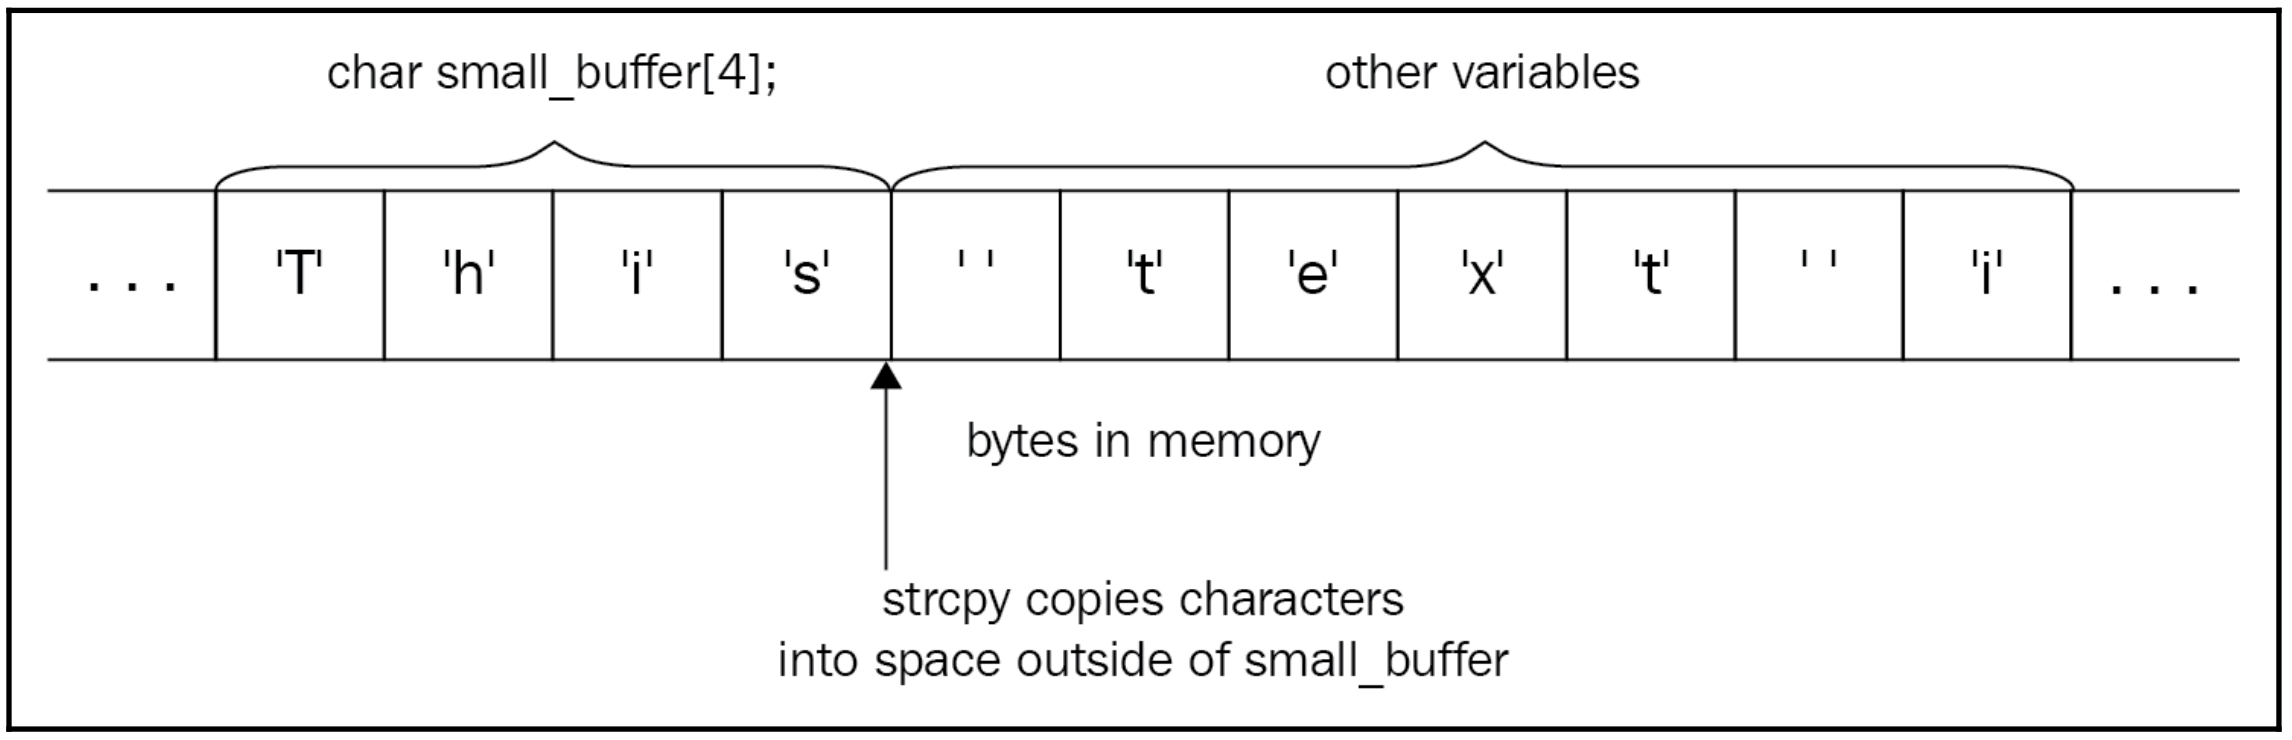
\includegraphics[width=1.0\textwidth]{content/Section-2/Chapter-12/13}
\end{center}

实现网络应用程序时,应该更加小心。大多数来自客户端连接的数据都应该得到正确的处理,缓冲区溢出的情况并不少见。让我们学习如何使网络应用程序更加安全。 \par

\noindent\textbf{}\ \par
\textbf{通信网络应用} \ \par
在本书的前一节中,我们设计了一个网络应用程序,它使用套接字连接接收客户端数据。除了大多数入侵系统的病毒来自外部世界这一事实之外,网络应用程序也有这种自然趋势,使计算机对Internet上的各种威胁敞开大门。首先,无论何时运行网络应用程序,系统中都存在一个开放的端口。知道应用程序正在监听的确切端口的人,可以通过伪造协议数据进行入侵。我们主要讨论的网络应用程序是在服务器端。但也有一些主题也适用于客户端应用。 \par
应该做的第一件事是合并客户端授权和身份验证,这两个术语很容易混淆。注意不要交替使用,它们是不同的: \par

\begin{itemize}
	\item 身份验证是验证客户端访问的过程。这意味着不是每个传入的连接请求都能立即得到服务。在与客户端之间传输数据之前,服务器应用程序必须确保客户端是已知的。与我们通过输入电子邮件和密码访问社交网络平台的方式相同,客户端的身份验证确定了客户端是否有权访问系统。
	\item 授权定义了客户端在系统中可以做什么。它是一组提供给特定客户端的权限。例如,我们在上一节中讨论的客户机应用程序能够向系统上传文件。你可能会想要加入付费订阅,并为付费客户提供更广泛的功能,例如:允许他们创建文件夹来组织文件。因此,当客户端请求创建文件夹时,我们可能希望授权请求,以确定客户端是否有权这样做。
\end{itemize}

当客户端应用程序发起与服务器的连接时,服务器获得的只是连接详细信息(IP地址、端口号)。为了让服务器知道谁是客户机应用程序(实际用户)的后台,客户机应用程序将发送用户的凭据。通常,这个过程包括向用户发送唯一标识符(如用户名或电子邮件地址)和密码,以访问系统。然后,服务器根据其数据库检查这些凭证,并验证是否应该授予对客户端的访问权。客户端和服务器之间的这种通信形式可能是简单的文本传输或格式化的对象传输。 \par
例如,由服务器定义的协议可能要求客户端以以下形式发送一个JavaScript对象符号(JSON)文档: \par

\begin{lstlisting}[caption={}]
{
	"email": "myemail@example.org",
	"password": "notSoSIMPLEp4s8"
}
\end{lstlisting}

来自服务器的响应允许客户机进一步进行或更新其UI,以让用户知道操作的结果。在登录时使用Web或网络应用程序时,可能会遇到几种情况。例如,输入错误的密码可能会导致服务器返回无效的用户名或密码错误。 \par
除了这第一个必要的步骤之外,验证来自客户机应用程序的每个数据片段是明智的。如果检查电子邮件字段的大小,则可以很容易地避免缓冲区溢出,例如:当客户端应用程序故意破坏系统时,可能会发送一个JSON对象,该对象的字段具有非常大的值。这是服务器的责任,防止安全缺陷需要从数据验证开始。 \par
另一种形式的安全攻击是每秒从单个或多个客户端发出太多请求,例如:一个客户端应用程序在一秒钟内发出数百个身份验证请求,这会导致服务器集中处理这些请求,并在试图为所有请求提供服务时浪费资源。最好检查客户机请求的速率,例如:将请求限制为每秒一个。 \par
这些形式的攻击(有意或无意的)称为拒绝服务(DOS)攻击。DOS攻击的更高级版本采取了从多个客户机向服务器发出大量请求的形式,这种形式称为分布式DOS(DDOS)攻击。一种简单的方法是,通过每秒发出多个请求来将试图使系统崩溃的IP地址列入黑名单。作为一名网络应用程序的开发者,在开发应用程序时,应该考虑到这里描述的所有问题以及本书范围之外的许多其他问题。 \par

\noindent\textbf{}\ \par
\textbf{总结} \  \par
本章中,我们介绍了用C++设计网络应用程序。C++23标准可能会支持。 \par                                                                                                                                                                                                                                                                                                                                                                                                                                                                                                                                                                                                                                                                                                                                                                                                                                                                                                                                                                                                                                                                                                                                                                                                                                                                                                                                    
我们首先介绍了网络的基础知识。完全理解网络需要花费大量时间,但在实现与网络相关的应用程序之前,有几个基本概念是每个开发者都必须了解的。这些基本概念包括OSI模型中的分层和不同类型的传输协议,如:TCP和UDP。对于开发者来说,理解TCP和UDP之间的差异都是必要的。正如我们所了解的,TCP在套接字之间建立可靠的连接,而套接字是程序员在开发网络应用程序时遇到的下一个问题。它们是应用程序的两个实例的连接点。当我们需要通过网络发送或接收数据时,我们应该定义一个套接字,并像处理常规文件一样处理它。 \par
我们在应用程序开发中使用的所有抽象和概念都由操作系统处理,最终由网络适配器处理。这是一种能够通过网络媒体发送数据的设备。从媒体接收数据并不能保证安全。网络适配器接收来自媒体的任何东西。为了确保正确地处理传入的数据,我们还应该注意应用的安全性。本章的最后一节是关于编写安全代码和验证输入,以确保不会对程序造成损害。程序安全是确保高质量程序的一个重要步骤。当然,确保程序无误的最佳方法是彻底测试它们。第10章中我们讨论了软件开发步骤,并解释了在编码阶段完成后对程序进行测试的重要性。测试之后,很可能会发现许多Bug。其中一些错误很难重现或修复,这就是调试的作用所在。 \par
下一章就来介绍一下正确的测试和如何调试程序。 \par

\noindent\textbf{}\ \par
\textbf{问题} \ \par
\begin{enumerate}
	\item 列出OSI模型的所有七个层。
	\item 端口号有什么意义?
	\item 为什么要在网络应用程序中使用套接字?
	\item 描述在服务器端执行的操作序列,以便使用TCP套接字接收数据。
	\item TCP和UDP之间的区别是什么?
	\item 为什么不应该在代码中使用宏定义?
	\item 实现服务器应用程序时,如何区分不同的客户机应用程序?
\end{enumerate}

\noindent\textbf{}\ \par
\textbf{扩展阅读} \ \par
\begin{itemize}
	\item TCP/IP Illustrated, Volume 1: The Protocols, by R. Stevens:  https:/​/​www.​amazon.com/​TCP-​Illustrated-​Protocols-​Addison-​Wesley-​Professional/​dp/0321336313/​ .
	\item Networking Fundamentals, by Gordon Davies: https://www.packtpub.com/cloud-networking/networking-fundamentals
\end{itemize}

\newpage








































